%%%%%%%%%%%%%%%%%%%%%%%%%%%%%%%%%%%%%%%%%%%%%%%%%%%%%%%%%%%%%%%%%%%%%%%
%%%% Содержание автореферата                                      %%%%
%%%%%%%%%%%%%%%%%%%%%%%%%%%%%%%%%%%%%%%%%%%%%%%%%%%%%%%%%%%%%%%%%%%%%%%

%%% Общая характеристика работы %%%
\pdfbookmark{Общая характеристика работы}{characteristic}
\section*{Общая характеристика работы}

\subsection*{Актуальность темы исследования}
\actualityText

\subsection*{Степень разработанности темы}
\degreeText

\subsection*{Цель работы}
\aimText

\subsection*{Задачи исследования}
\tasksText

\subsection*{Методология и методы исследования}
\methodsText

\subsection*{Объект исследования}
\objectText

\subsection*{Предмет исследования}
\subjectText

\subsection*{Научная новизна}
\noveltyText

\subsection*{Теоретическая значимость}
\theoreticalText

\subsection*{Практическая значимость}
\influenceText

\subsection*{Положения, выносимые на защиту}
\defpositionsText

\subsection*{Соответствие диссертации паспорту научной специальности}
\conformityText

\subsection*{Достоверность полученных результатов}
\reliabilityText

\subsection*{Апробация работы}
\probationText

\subsection*{Личный вклад автора}
\contributionText

\subsection*{Публикации}
\publicationsText

%%% Содержание работы %%%
\pdfbookmark{Содержание работы}{description}
\section*{Содержание работы}

Во \textbf{введении} обоснована актуальность темы, сформулирована цель
исследования - повышение эффективности процессов распознавания
и~реидентификации людей в~ИПС - и~определены задачи, решение которых
обеспечивает достижение поставленной цели. Приведены методология и~методы исследования, раскрыты научная
новизна, теоретическая и~практическая значимость, сформулированы положения,
выносимые на~защиту.

Отдельно подчеркнута специфика функционирования ИПС в~условиях
информационной неопределенности: неполной доступности отдельных модальностей,
вариативности их внешнего вида и~<<каскадного эффекта>> ошибок
последовательных этапов обработки. Это обосновывает
необходимость комплексного подхода, обеспечивающего согласованную
оптимизацию всех стадий контура обработки данных.

\subsection*{Первая глава}

В~\textbf{первой главе} выполнен анализ теоретических основ распознавания
сложных объектов и~рассмотрено место задачи реидентификации (на~примере
личности) в~составе информационно-поисковых систем. Проведена
систематизация подходов к~анализу высокоинформативных, но~уязвимых
признаков (на~примере лица) и~более устойчивых, но~менее дискриминативных
признаков (силуэт, атрибуты, контекст). Показано, что в~практических
сценариях ни~одна из~модальностей не~является гарантированно надежной:
ключевые модальности могут быть недоступны из-за окклюзий, низкого
разрешения или неблагоприятного ракурса наблюдения. На~основе анализа
фундаментальных работ (включая методы М.~Терка, А.~Пентланда и~др.)
обоснована необходимость многофакторных решений, интегрирующих
комплементарные источники признаков.

Рассмотрены современные постановки задач визуального поиска объекта
в~массиве данных при ограничениях по~времени ответа и~вычислительным
ресурсам. Показано, что типовые информационные процессы в~ИПС строятся
как последовательность этапов: (1)~получение и~предобработка данных,
(2)~детектирование связанных объектов <<силуэт-лицо>>, (3)~ассоциация
наблюдений (трекинг), (4)~формирование признаковых представлений
(эмбеддингов), (5)~интеграция источников признаков и~принятие решения,
(6)~выдача результата и~протоколирование. Качество итогового распознавания
определяется согласованностью всех перечисленных процессов, а~ошибки
на~ранних стадиях приводят к~каскадной деградации результата. Место
предлагаемых в~работе улучшений в~общем контуре обработки данных
представлено на~рис.~\ref{fig:reid-scheme}.

\begin{figure}[H]
\centering
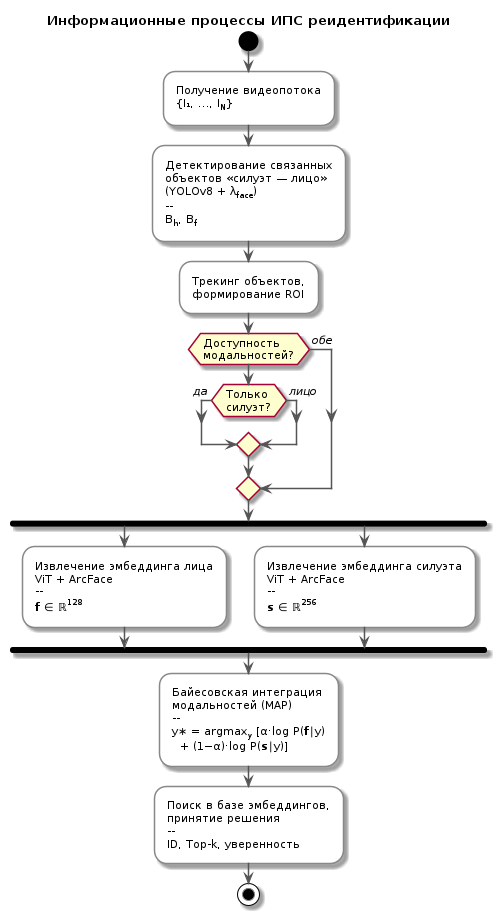
\includegraphics[width=0.55\textwidth,height=0.7\textheight,keepaspectratio]{images/1.png}
\caption{Схема информационных процессов ИПС реидентификации личности и~место
разработанных решений}
\label{fig:reid-scheme}
\end{figure}

Для формального описания контура обработки данных введены множества
и~отображения, задающие процесс распознавания/реидентификации в~ИПС.
Дано множество изображений (кадров) видеопотока:
\begin{equation}
    \mathcal{I}=\{I_i\}_{i=1}^{N_I},
    \label{eq:images}
\end{equation}
где каждое изображение $I_i$ содержит одного или нескольких людей.

Определены функции детектирования: функция детектирования силуэта (человека)
$D_h(\cdot)$, возвращающая множество ограничивающих рамок (силуэтов) $B_h$
для изображения~$I$; функция детектирования лица $D_f(\cdot)$, возвращающая
множество ограничивающих рамок лиц~$B_f$ для изображения~$I$ или пустое множество,
если лицо не~обнаружено; функция извлечения признаков (эмбеддинга) $\Phi(\cdot)$,
преобразующая детектированный объект (силуэт или лицо) в~вектор признаков заданной
размерности.

Необходимо определить правило объединения признаков двух модальностей,
позволяющее использовать доступные наблюдения в~условиях неполноты данных.
Вводится функция комбинирования $g(\cdot)$, формирующая комбинированный вектор
признаков~$\mathbf{z}$ на~основе вектора силуэта~$\mathbf{s}$ и~вектора
лица~$\mathbf{f}$:
\begin{equation}
    \mathbf{z}=g(\mathbf{s},\mathbf{f}).
    \label{eq:combination}
\end{equation}

Функционирование ИПС в~рамках решаемой задачи формализуется как последовательность
информационных процессов, которая для каждого входного изображения~$I$ выполняет
следующие шаги.

1)~Детектирование силуэта и~лица на~изображении~$I$:
\begin{equation}
    B_h=D_h(I),\quad B_f=D_f(I).
    \label{eq:detection}
\end{equation}

2)~Преобразование детектированных объектов в~векторы признаков с~помощью функции
$\Phi(\cdot)$. Для выбранных детекций (например, наиболее вероятных по~score либо
согласованных с~трекингом) выделяются области интереса (region of interest, ROI),
по~которым вычисляются эмбеддинги:
\begin{equation}
    \mathbf{s}=\Phi(\mathrm{ROI}_{human}),
    \label{eq:emb-human}
\end{equation}
\begin{equation}
    \mathbf{f}=\Phi(\mathrm{ROI}_{face}).
    \label{eq:emb-face}
\end{equation}

3)~Комбинирование векторов для получения интегрального описания наблюдаемого
объекта согласно~(\ref{eq:combination}).

4)~Идентификация/реидентификация по~базе эмбеддингов (или по~индексу ИПС),
то~есть вычисление решающей функции $A(\cdot)$, которая по~вектору~$\mathbf{z}$
и~базе~$\mathrm{DB}$ возвращает идентификатор, оценку уверенности и/или
ранжированный список кандидатов.

В~предлагаемой методике обозначение $\mathbf{z}$ используется как интегральное
признаковое описание наблюдаемого объекта: в~базовом варианте $\mathbf{z}$ является
комбинированным вектором признаков (например, при линейном объединении эмбеддингов),
а~в~вероятностном варианте интеграции $\mathbf{z}$ соответствует паре наблюдений
$(\mathbf{f},\mathbf{s})$, используемой в~решающем правиле $A(\cdot)$.
Далее функция комбинирования $g(\cdot)$ и~решающая функция $A(\cdot)$ реализуются
через байесовскую интеграцию модальностей и~MAP‑критерий (гл.~2), что обеспечивает
интерпретируемое принятие решений и~корректную работу при неполноте данных.

Цель - минимизировать ошибку реидентификации при оптимальных вычислительных
затратах за~счет согласованной оптимизации качества выделения связанных
объектов <<силуэт-лицо>> (детектирование), дискриминативности признакового
описания каждой модальности (эмбеддинги) и~корректности правила
вероятностной интеграции при принятии решения.

\subsection*{Вторая глава}

Во \textbf{второй главе} изложены теоретические результаты, составляющие
разработанную комплексную методику и~соответствующие трем положениям,
выносимым на~защиту.

\textbf{Структура комплексной методики.} Разработанная методика реализует
единый конвейер обработки видеокадра в~ИПС и~состоит из~четырех
последовательных этапов:
\begin{enumerate}
    \item согласованное детектирование связанных объектов <<силуэт-лицо>>;
    \item раздельное извлечение дискриминативных эмбеддингов лица
          и~силуэта;
    \item вычисление гауссовых правдоподобий для каждого класса
          личности;
    \item принятие решения по~многоклассовому MAP-критерию.
\end{enumerate}
Высокоуровневая схема методики и~место предлагаемых улучшений в~контуре
обработки данных представлены на~рис.~\ref{fig:reid-scheme}; формальная
постановка приведена в~гл.~1, выражения~(\ref{eq:images})--(\ref{eq:combination}).
Каждый из~этапов методики реализован за~счет соответствующего метода,
выносимого на~защиту (табл.~\ref{tab:method-mapping}). Поэтапная
декомпозиция обеспечивает целенаправленное повышение качества
на~каждой стадии и~минимизирует каскадный эффект накопления ошибок.

\begin{table}[H]
\centering
\caption{Соответствие этапов комплексной методики методам, выносимым
на~защиту}
\label{tab:method-mapping}
\resizebox{\textwidth}{!}{%
\begin{tabular}{c|l|c|l}
\hline
Этап & Содержание этапа & Положение & Формулы \\
\hline
1 & Согласованное детектирование <<силуэт-лицо>>           & 1 & (\ref{eq:detection}), (\ref{eq:loss}) \\
2 & Извлечение эмбеддингов (ViT + ArcFace + $L_2$)         & 2 & (\ref{eq:emb-human}), (\ref{eq:emb-face}) \\
3 & Гауссовы правдоподобия $P(\mathbf{f}\mid y)$, $P(\mathbf{s}\mid y)$ & 3 & (\ref{eq:gauss}) \\
4 & MAP-решение                                            & 3 & (\ref{eq:map})--(\ref{eq:map-only-f}) \\
\hline
\end{tabular}}
\end{table}

Далее в~подразделах изложены разработка и~обоснование каждого
из~методов, реализующих этапы методики.

\textit{Первый результат} (положение~1) относится к~процессу
согласованного детектирования связанных объектов <<силуэт-лицо>>. В~качестве базовой модели выбран детектор YOLOv8.
Ключевым достоинством данной архитектуры является сбалансированное сочетание
высокой скорости обработки (режим реального времени) и~точности локализации
за~счет использования эффективных блоков C2f и~механизма Spatial Pyramid
Pooling Fast (SPPF). Показано, что при решении задачи реидентификации важно
не~только обнаружение человека как объекта класса <<силуэт>>, но~и~корректное
обнаружение лица, находящегося внутри силуэта, поскольку именно лицо
при наличии обеспечивает высокую дискриминативность при сравнении
личностей. При использовании стандартного критерия обучения детектора
вклад ошибок детекции лиц в~суммарный функционал обучения может быть
недостаточным по~сравнению с~вкладом ошибок детекции силуэта, что ухудшает
качество формирования ROI лица для последующих этапов ReID в~сценариях
с~плотной сценой, окклюзиями и~вариативным ракурсом лица.

Для усиления чувствительности детектора к~ошибкам обнаружения лиц,
ассоциированных с~силуэтом, предложена модификация функции потерь YOLOv8:
в~стандартный критерий $\mathcal{L}_0$ введен дополнительный компонент
$\mathcal{L}_{\text{face}}$, учитывающий ошибки детекции лиц в~пределах
ограничивающих рамок силуэта, и~коэффициент~$\lambda_{\text{face}}$,
регулирующий вклад данного компонента. Итоговая функция потерь имеет вид:
\begin{equation}
    \mathcal{L}=\mathcal{L}_0+\lambda_{\text{face}}\,
    \frac{1}{N_{\text{pred}}}\sum_{i=1}^{N_{\text{pred}}}\mathbb{I}_{\text{face}}(i)\,
    \mathcal{L}_{\text{face}}(i),
    \label{eq:loss}
\end{equation}
где $\mathcal{L}_0$~- исходная функция потерь модели YOLOv8;
$N_{\text{pred}}$~- общее число предсказаний, соответствующих объектам;
$\mathbb{I}_{\text{face}}(i)$~- индикаторная функция, принимающая значение~1,
если $i$-я ячейка содержит лицо, и~0~- в~противном случае;
$\mathcal{L}_{\text{face}}(i)$~- добавочный штраф за~ошибку локализации
лица относительно границ силуэта; $\lambda_{\text{face}}$~- управляющий
коэффициент, определяющий вес лицевого члена в~суммарном функционале. Показано, что введение
коэффициента~$\lambda_{\text{face}}$ позволяет управлять компромиссом между
качеством детекции лиц и~стабильностью качества детекции класса <<силуэт>>,
что особенно важно для последующих этапов извлечения признаков и~принятия
решения в~ИПС. Структура базового детектора YOLOv8, используемого
на~этапе детектирования, показана на~рис.~\ref{fig:yolov8}.

\begin{figure}[H]
\centering
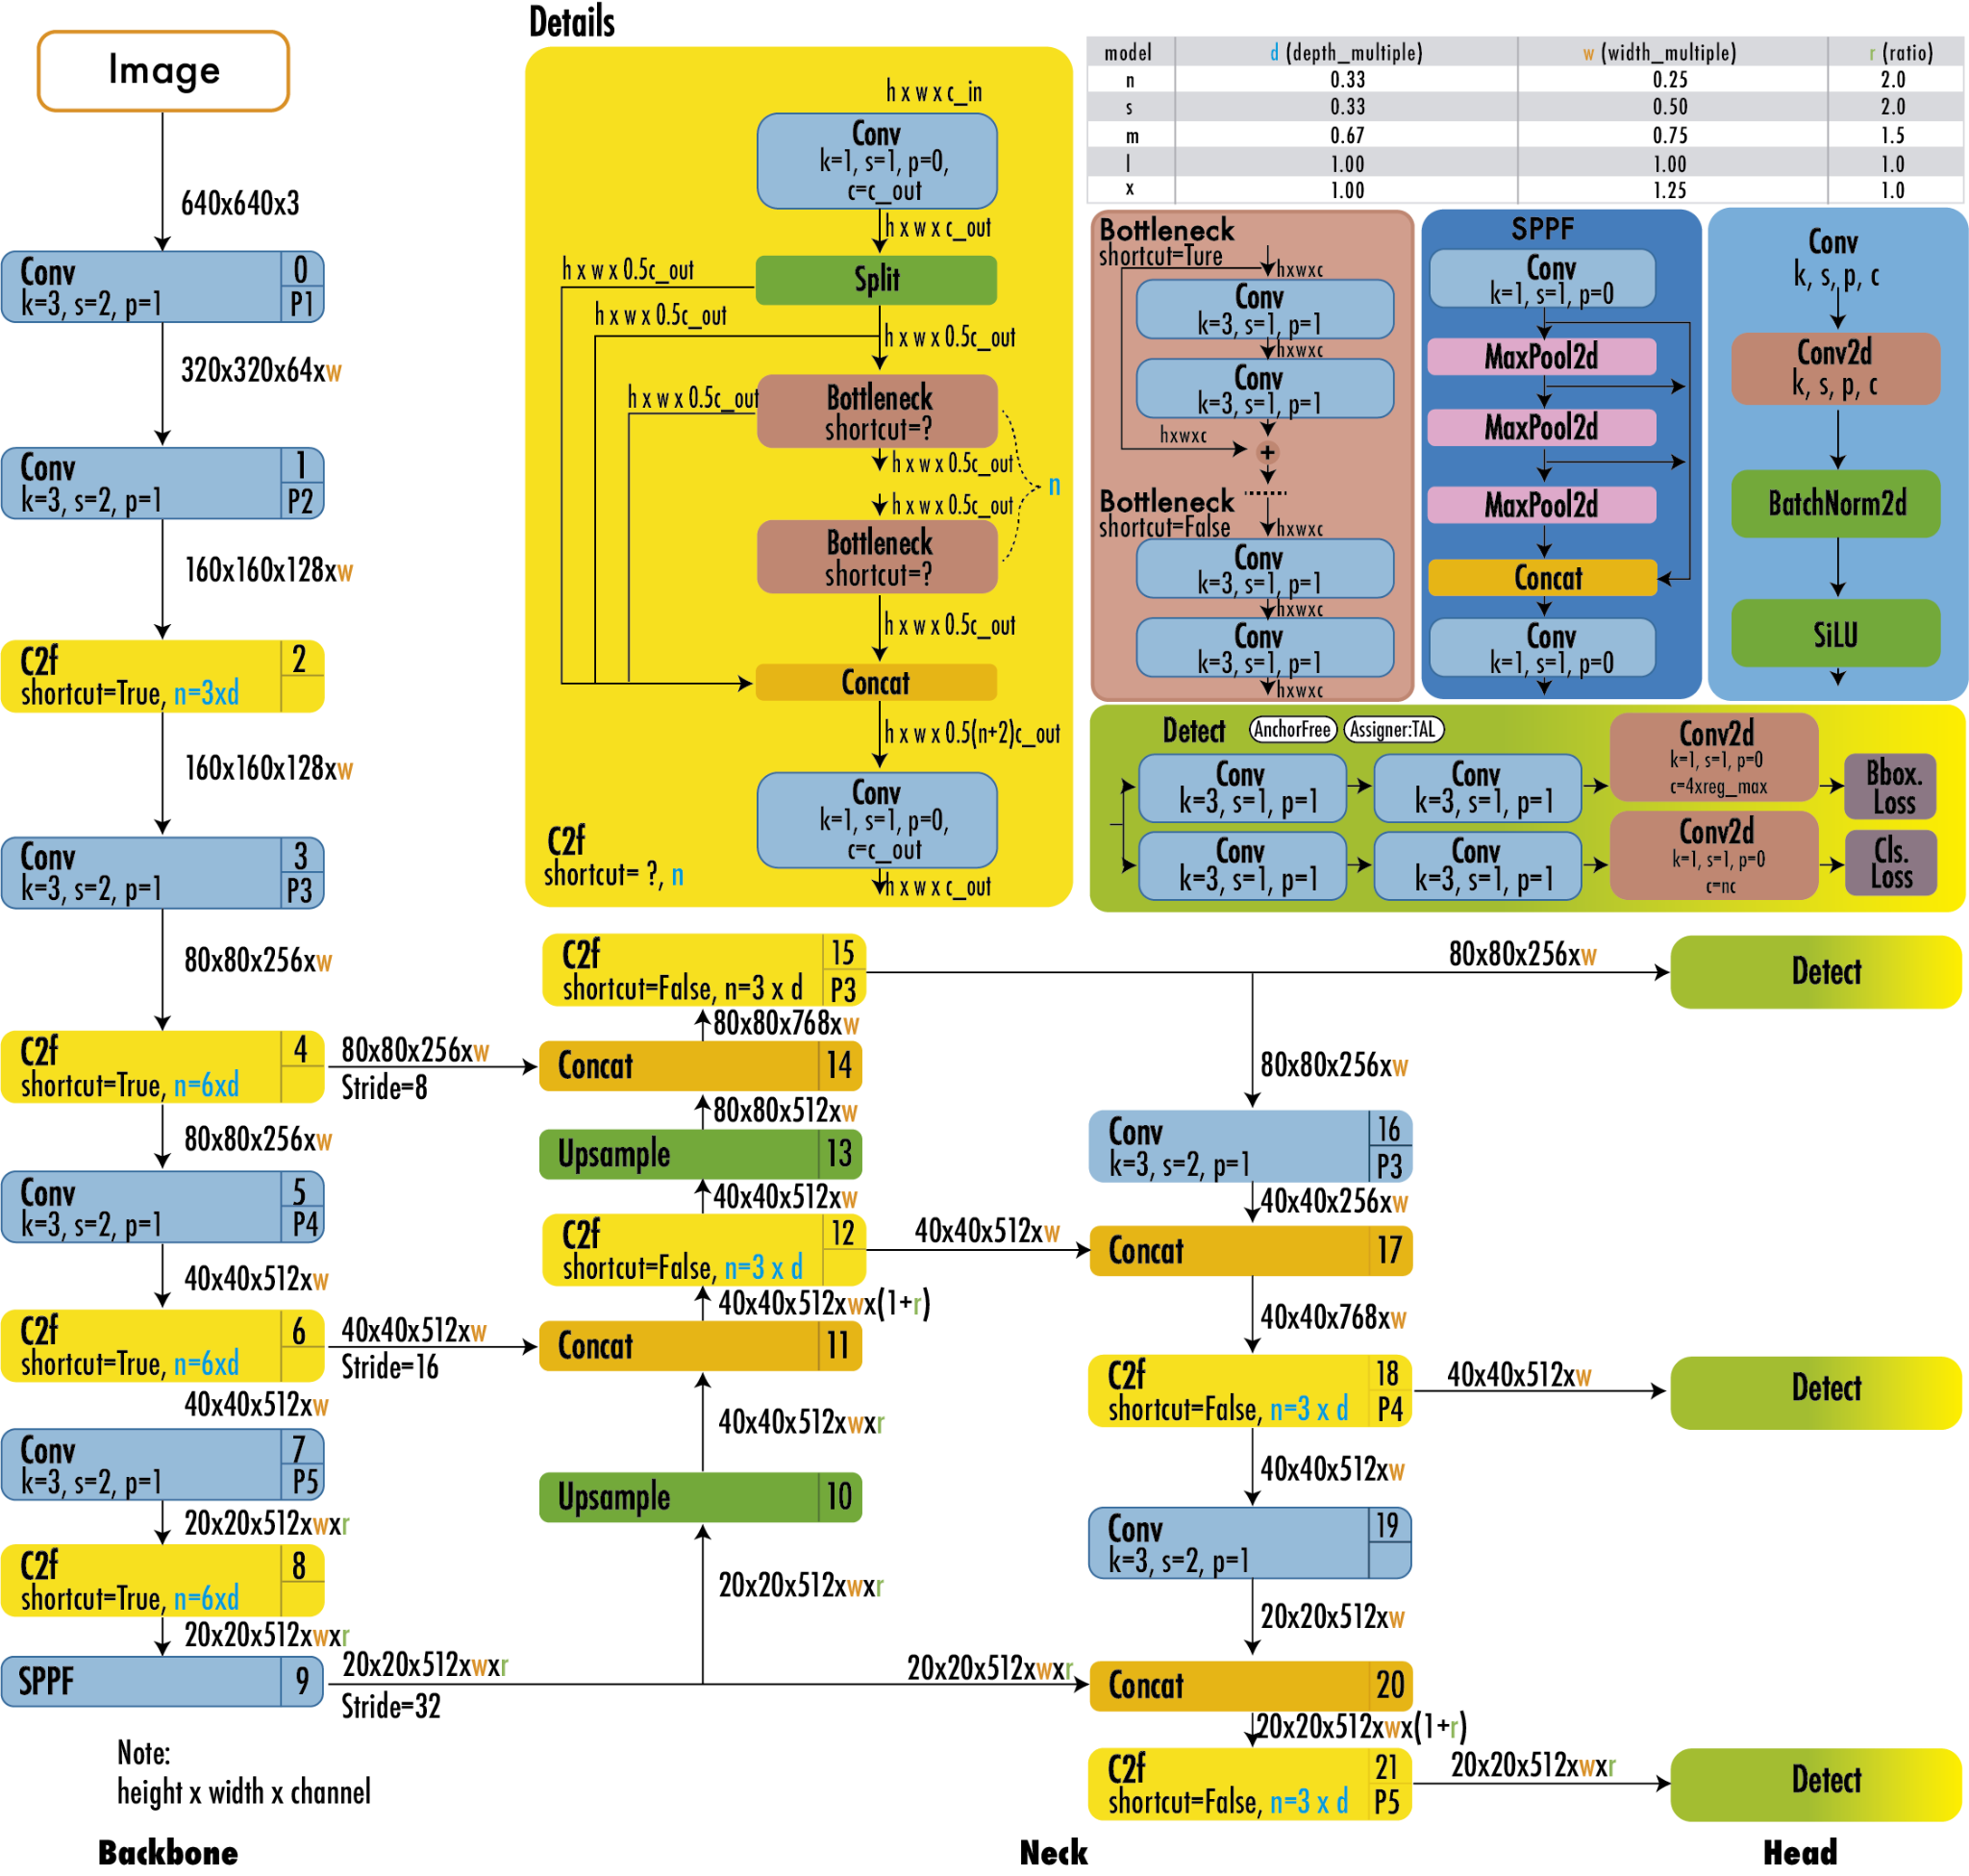
\includegraphics[width=0.8\textwidth,height=0.8\textheight,keepaspectratio]{images/2.png}
\caption{Схема архитектуры YOLOv8}
\label{fig:yolov8}
\end{figure}

\textit{Второй результат} (положение~2) относится к~процессу формирования
признаковых представлений (эмбеддингов) для лицевой и~силуэтной модальностей.
Показано, что задача ReID в~ИПС является многофакторной: устойчивость решения
определяется не~только наличием <<наиболее информативной>> модальности,
но~и~способностью системы работать при частичном отсутствии данных. Поэтому
предложен метод формирования дискриминативных эмбеддингов лица и~силуэта,
ориентированный на~совместимое использование этих представлений на~следующем
этапе интеграции.

Метод включает: (1)~формирование ROI лица и~ROI силуэта по~результатам
детектирования и~трекинга; (2)~извлечение векторных представлений двумя
специализированными ViT-кодировщиками; (3)~обучение кодировщиков
на~множестве классов личности с~использованием функции потерь ArcFace,
обеспечивающей
формирование выраженных межклассовых границ в~эмбеддинг‑пространстве;
(4)~нормировку эмбеддингов ($L_2$‑нормировка), обеспечивающую корректность
и~устойчивость последующих сравнений и~вероятностных оценок.

Принципиально важно, что в~рамках метода эмбеддинги формируются раздельно
для каждой модальности (лицо и~силуэт). Такая раздельная схема:
\begin{itemize}
    \item обеспечивает использование более дискриминативной модальности
          (лицо) при~ее доступности;
    \item компенсирует отсутствие или низкое качество лицевой модальности
          за~счет более часто доступной силуэтной модальности;
    \item обеспечивает совместимость эмбеддингов с~вероятностной моделью
          интеграции (положение~3) за~счет стандартизации представлений
          и~нормировки.
\end{itemize}

\textit{Третий результат} (положение~3) относится к~процессу вероятностной
интеграции признаков лицевой и~силуэтной модальностей и~принятия решения
о~личности наблюдаемого человека. Рассмотрены распространенные
подходы multimodal fusion (конкатенация, линейное объединение эмбеддингов,
fusion на~уровне оценок, attention-механизмы, графовые модели) и~отмечены
их ограничения в~эксплуатационных режимах ИПС: необходимость ручной настройки
весов и~ухудшение поведения при исчезновении одной из~модальностей. В~этой
связи предложена явная байесовская модель интеграции лицевых и~силуэтных
эмбеддингов с~MAP-решающим правилом.

Задача распознавания моделируется как статистическая классификация
личности~$y$ по~двум наблюдениям: вектору признаков лица~$\mathbf{f}$
и~вектору признаков силуэта~$\mathbf{s}$. Пусть $y$~- дискретная случайная
переменная, принимающая значения из~множества классов~$Y$. При допущении
условной независимости наблюдений $\mathbf{f}$ и~$\mathbf{s}$ при
фиксированном классе~$y$ апостериорная вероятность принадлежности
наблюдений $(\mathbf{f},\mathbf{s})$ классу~$y$ определяется по~теореме
Байеса:
\begin{equation}
    P(y\mid \mathbf{f},\mathbf{s})=
    \frac{P(\mathbf{f}\mid y)\,P(\mathbf{s}\mid y)\,P(y)}
    {\sum\limits_{y'\in Y}P(\mathbf{f}\mid y')\,P(\mathbf{s}\mid y')\,P(y')}.
    \label{eq:bayes}
\end{equation}

В~условиях непредвзятой идентификации априорные вероятности кандидатов
принимаются равными, $P(y)=\mathrm{const}$. Тогда правило принятия решения
имеет вид MAP‑критерия; для повышения численной устойчивости используется
логарифмирование правдоподобий:
\begin{equation}
    y^*=\arg\max\limits_{y\in Y}
    \left[\log P(\mathbf{f}\mid y)+\log P(\mathbf{s}\mid y)\right].
    \label{eq:map}
\end{equation}

Выражение~(\ref{eq:map}) показывает, что решение формируется как сумма двух
<<свидетельств>>~- от~лица и~от~силуэта. Если одна из~модальностей отсутствует
либо ненадежна, ее вклад в~правдоподобие становится малым, и~решение
принимается преимущественно на~основе другой модальности, что обеспечивает
корректное поведение ИПС при неполноте данных. При низком качестве одной
из~модальностей соответствующее правдоподобие становится менее информативным
(ближе к~равномерному по~кандидатам), поэтому вклад этой модальности
в~критерий максимизации уменьшается, и~решение определяется преимущественно
другой модальностью.

Если при обработке кадра лицо не~обнаружено ($B_f=\varnothing$) и~эмбеддинг
$\mathbf{f}$ отсутствует, то~MAP-правило редуцируется к~одномодальному случаю:
\begin{equation}
    y^*=\arg\max\limits_{y\in Y}\log P(\mathbf{s}\mid y).
    \label{eq:map-only-s}
\end{equation}
Аналогично, при отсутствии силуэтной модальности используется только
$\mathbf{f}$:
\begin{equation}
    y^*=\arg\max\limits_{y\in Y}\log P(\mathbf{f}\mid y).
    \label{eq:map-only-f}
\end{equation}

Для вычисления $P(\mathbf{f}\mid y)$ и~$P(\mathbf{s}\mid y)$ используется
вероятностная модель распределения эмбеддингов каждой модальности для каждой
личности. В~исследовании применяется модель многомерного нормального
распределения в~пространстве эмбеддингов. Для модальности лица
предполагается:
\begin{equation}
    P(\mathbf{f}\mid y)=
    \frac{1}{(2\pi)^{d/2}\,|\Sigma_y|^{1/2}}
    \exp\!\left(-\frac{1}{2}(\mathbf{f}-\boldsymbol{\mu}_y)^T
    \Sigma_y^{-1}(\mathbf{f}-\boldsymbol{\mu}_y)\right),
    \label{eq:gauss}
\end{equation}
и~аналогично для $P(\mathbf{s}\mid y)$ со~своими параметрами в~пространстве
силуэта. Здесь $\boldsymbol{\mu}_y$~- средний вектор (центроид) признаков
класса~$y$ в~соответствующем пространстве, $\Sigma_y$~- ковариационная
матрица, отражающая разброс признаков внутри класса; обе величины
оцениваются по~обучающей выборке отдельно для лицевой и~силуэтной
модальностей. Размерность пространства эмбеддингов: $d=128$ для лица
и~$d_s=256$ для силуэта. Использование такой модели позволяет учитывать,
что лицевая и~силуэтная модальности обладают различной вариативностью
(например, признаки одежды меняются чаще, чем черты лица). Применение диагональной
или изотропной ковариации позволяет снизить число параметров и~повысить
устойчивость оценивания при ограниченном числе образцов на~класс.

Важной особенностью MAP-правила~(\ref{eq:map}) является автоматическое
взвешивание модальностей через ковариационные матрицы~$\Sigma_y$ гауссовых
правдоподобий. В~логарифме правдоподобия
$\log P(\mathbf{x}\mid y) = -\tfrac{1}{2}\!\left[(\mathbf{x}-\boldsymbol{\mu}_y)^{T}\Sigma_y^{-1}(\mathbf{x}-\boldsymbol{\mu}_y)+\log|\Sigma_y|+d\log 2\pi\right]$
расстояние Махаланобиса содержит обратную ковариацию~$\Sigma_y^{-1}$:
модальность с~меньшей внутриклассовой дисперсией (более компактными
кластерами личностей в~признаковом пространстве) дает более <<острое>>
правдоподобие и~автоматически доминирует в~argmax. Тем самым адаптивный
вклад каждой модальности достигается без ручной подстройки весов
и~без введения дополнительного гиперпараметра комбинирования: роль
коэффициентов доверия здесь играют ковариационные матрицы~$\Sigma_y$,
оцениваемые по~обучающей выборке.

Обобщенная блок-схема предлагаемого метода байесовской реидентификации
приведена на~рис.~\ref{fig:bayes-scheme}.

\begin{figure}[H]
\centering
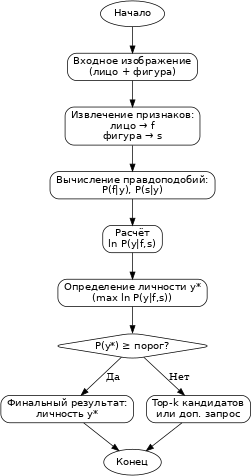
\includegraphics[width=0.5\textwidth,height=0.7\textheight,keepaspectratio]{images/3.png}
\caption{Блок‑схема предлагаемого метода байесовской реидентификации}
\label{fig:bayes-scheme}
\end{figure}

Таким образом, во~второй главе сформирована единая логическая цепочка
реидентификации людей: модифицированный критерий обучения детектора
повышает качество согласованной локализации связанных объектов
<<силуэт-лицо>> (положение~1); метод формирования дискриминативных
эмбеддингов обеспечивает устойчивые векторные представления для каждой
модальности изолированно (положение~2); байесовская модель интеграции
и~многоклассовое MAP-решение обеспечивают корректное объединение
лицевых и~силуэтных эмбеддингов и~принятие решения о~личности
наблюдаемого человека при неполноте данных (положение~3).

\subsection*{Третья глава}

В~\textbf{третьей главе} приведена экспериментальная проверка разработанных
теоретических решений. Эксперименты структурированы по~трем ключевым этапам
предложенной методики: оценка модифицированной функции потерь детектора
связанных объектов <<силуэт-лицо>>, оценка качества формируемых эмбеддингов
и~оценка итогового качества реидентификации при байесовской интеграции
лицевых и~силуэтных эмбеддингов.

Для оценки использованы стандартные в~задаче ReID наборы
данных CUHK03, Market-1501 и~MARS, обеспечивающие проверку работы алгоритмов
в~условиях сильного изменения ракурсов, освещенности и~окклюзий.

Вычислительные эксперименты проводились на~высокопроизводительном сервере;
его характеристики приведены в~табл.~\ref{tab:server} и~обеспечили обработку
больших массивов визуальных данных в~приемлемое время.

\begin{table}[H]
\centering
\caption{Характеристики серверной инфраструктуры для проведения вычислительных
экспериментов}
\label{tab:server}
\resizebox{0.75\textwidth}{!}{%
\begin{tabular}{ll}
\hline
Параметр & Характеристика \\
\hline
Операционная система & Ubuntu 22.04.4 LTS x86\_64 \\
Процессор (CPU) & AMD Ryzen 9 7950X (32 ядра, 5.88 GHz) \\
Графические процессоры & 2 $\times$ NVIDIA GeForce RTX 3090 Ti (24 ГБ) \\
Оперативная память (RAM) & 128 ГБ \\
Версия NVIDIA Driver & 555.42.02 \\
Версия CUDA & 12.5 \\
\hline
\end{tabular}}
\end{table}

\textit{Эксперименты по~положению~1.} Выполнена подготовка данных и~обучение
модифицированной модели YOLOv8 для согласованного выделения связанных
объектов <<силуэт-лицо>>. Экспериментально исследовано влияние коэффициента
$\lambda_{\text{face}}$ на~показатели качества детекции лица (класс
<<лицо>>) и~силуэта (класс <<силуэт>>). Варьирование
$\lambda_{\text{face}}$ выполнялось в~диапазоне от~0,1 до~2,7 при фиксированных
настройках обучения и~неизменной архитектуре детектора. Зависимости метрик
качества детектирования от~коэффициента~$\lambda_{\text{face}}$ представлены
на~рис.~\ref{fig:lambda-graphs}.

\begin{figure}[H]
\centering
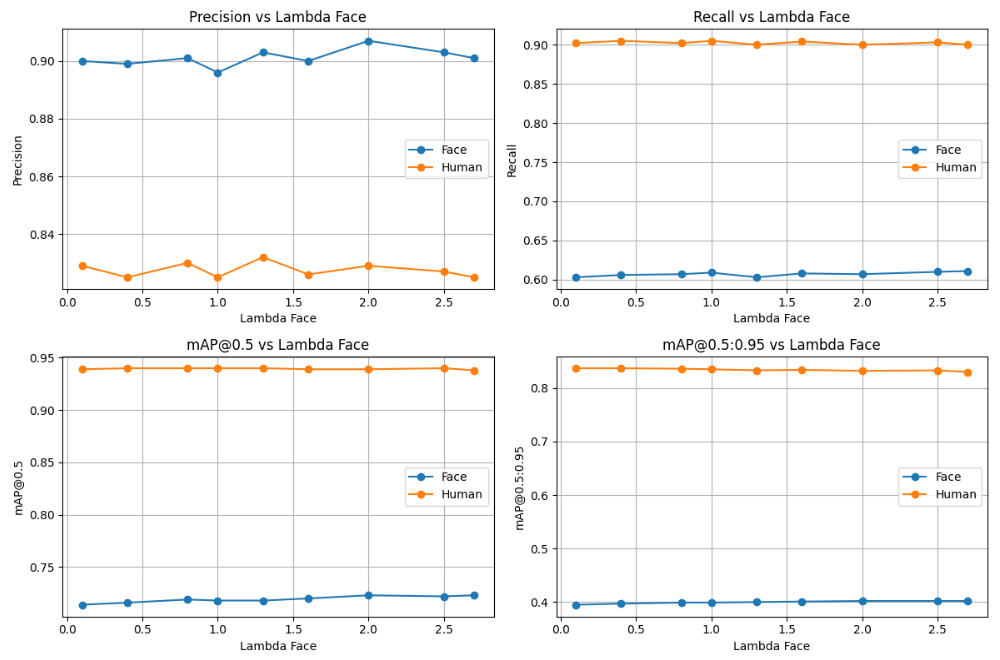
\includegraphics[width=0.8\textwidth]{images/4.png}
\caption{Графики зависимостей показателей качества детекции
от~$\lambda_{\text{face}}$}
\label{fig:lambda-graphs}
\end{figure}

Для анализа структуры ошибок детектирования для выбранных настроек
приведена матрица ошибок (рис.~\ref{fig:confusion-matrix}), демонстрирующая
снижение доли пропусков для малых объектов внутри ROI основной структуры.

\begin{figure}[H]
\centering
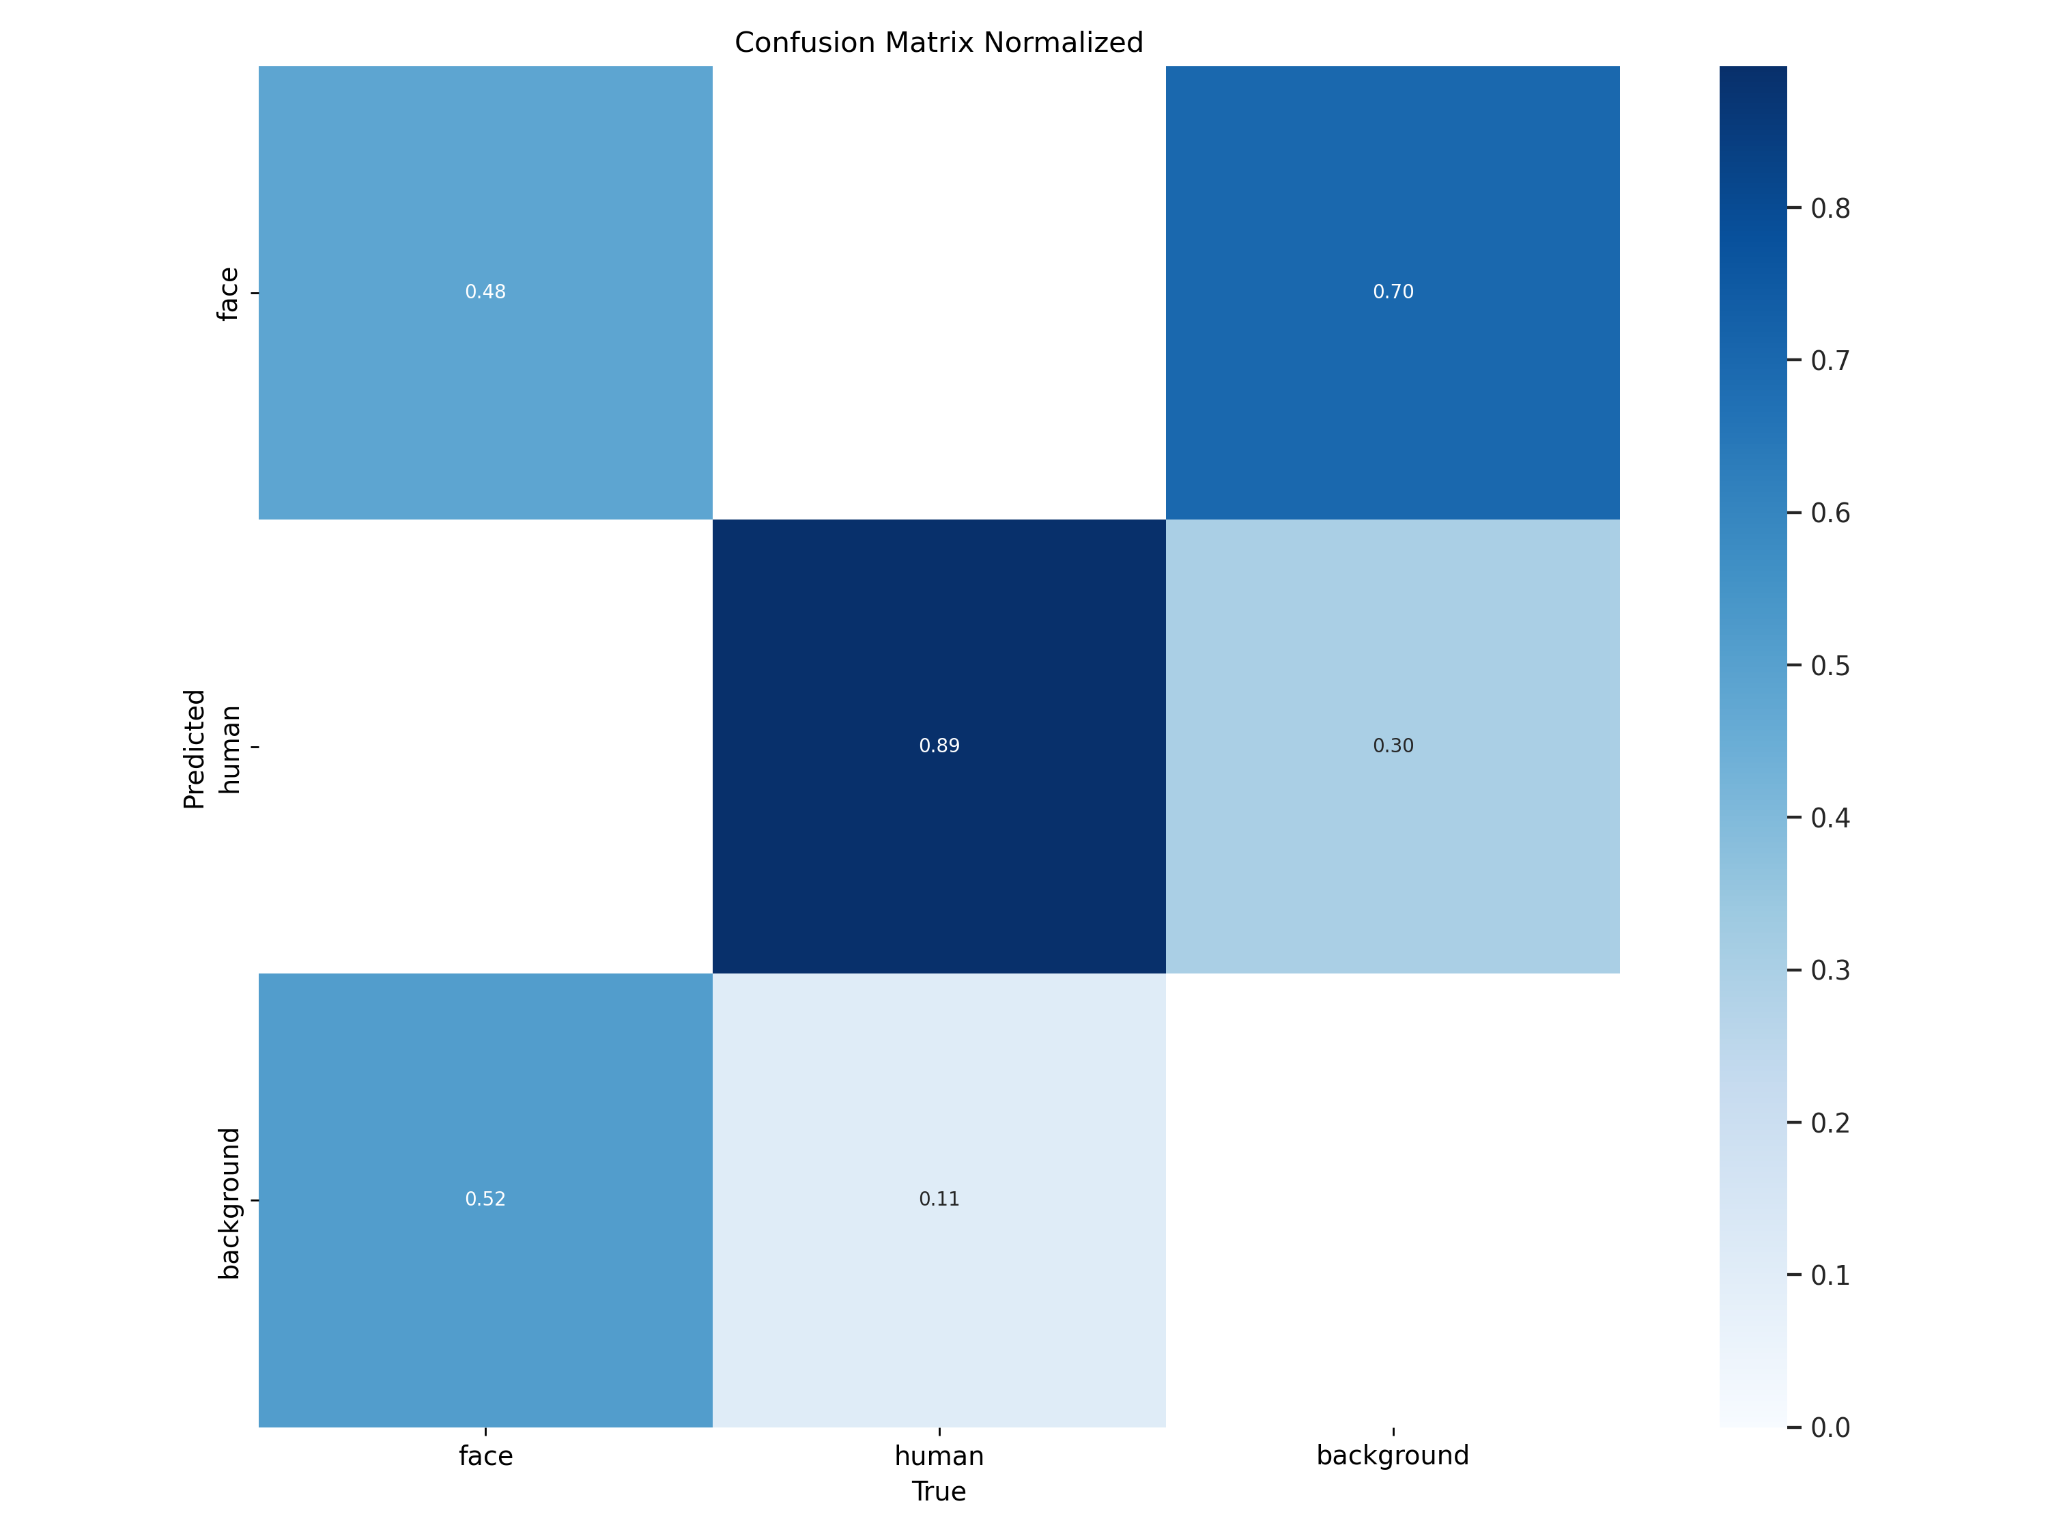
\includegraphics[width=0.9\textwidth]{images/5.png}
\caption{Матрица ошибок}
\label{fig:confusion-matrix}
\end{figure}

Численные значения метрик качества детектирования при варьировании
$\lambda_{\text{face}}$ приведены в~табл.~\ref{tab:lambda-face}.

\begin{table}[H]
\centering
\caption{Влияние коэффициента $\lambda_{\text{face}}$ на~качество детектирования
классов <<лицо>> и~<<силуэт>>}
\label{tab:lambda-face}
\resizebox{\textwidth}{!}{%
\begin{tabular}{c|cccc|cccc}
\hline
 & \multicolumn{4}{c|}{Класс <<лицо>>} & \multicolumn{4}{c}{Класс <<силуэт>>} \\
$\lambda_{\text{face}}$ &
Precision & Recall & mAP@0.5 & mAP@0.5:0.95 &
Precision & Recall & mAP@0.5 & mAP@0.5:0.95 \\
\hline
0,1 & 0,900 & 0,603 & 0,714 & 0,395 & 0,829 & 0,902 & 0,939 & 0,837 \\
0,4 & 0,899 & 0,606 & 0,716 & 0,397 & 0,825 & 0,905 & 0,940 & 0,837 \\
0,8 & 0,901 & 0,607 & 0,719 & 0,399 & 0,830 & 0,902 & 0,940 & 0,836 \\
1,0 & 0,896 & 0,609 & 0,718 & 0,399 & 0,825 & 0,905 & 0,940 & 0,835 \\
1,3 & 0,903 & 0,603 & 0,718 & 0,400 & 0,832 & 0,900 & 0,940 & 0,833 \\
1,6 & 0,900 & 0,608 & 0,720 & 0,401 & 0,826 & 0,904 & 0,939 & 0,834 \\
2,0 & 0,907 & 0,607 & 0,723 & 0,402 & 0,829 & 0,900 & 0,939 & 0,832 \\
2,5 & 0,903 & 0,610 & 0,722 & 0,402 & 0,827 & 0,903 & 0,940 & 0,833 \\
2,7 & 0,901 & 0,611 & 0,723 & 0,402 & 0,825 & 0,900 & 0,938 & 0,830 \\
\hline
\end{tabular}}
\end{table}

Характерные примеры работы модифицированного детектора в~типовых и~сложных
сценах приведены на~рис.~\ref{fig:detector-examples} (для корректного
тиражирования автореферата изображения подготовлены в~градациях серого).

\begin{figure}[H]
\centering

\includegraphics[width=0.9\textwidth]{images/6.png}
\caption{Примеры работы модифицированного детектора (в~градациях серого)}
\label{fig:detector-examples}
\end{figure}

Экспериментально установлено, что значения $\lambda_{\text{face}}$
в~диапазоне 2,0--2,7 обеспечивают максимальные показатели по~детекции лиц
без существенной деградации по~классу <<силуэт>>, что подтверждает
работоспособность предложенной модификации критерия обучения.

\textit{Эксперименты по~положению~2.} Проведена качественная оценка
эмбеддингов, сформированных предложенным методом независимо для двух
модальностей. Для анализа структуры признаковых пространств
использована визуализация методом t-SNE: отдельно для эмбеддингов лиц
(рис.~\ref{fig:tsne-face}) и~отдельно для эмбеддингов силуэтов
(рис.~\ref{fig:tsne-silhouette}). Для сопоставления с~базовыми
эвристическими способами объединения признаков выполнена визуализация
для линейного сложения векторов (рис.~\ref{fig:tsne-linear}). Визуальный
анализ подтверждает, что использование ViT и~ArcFace формирует выраженную
кластеризацию по~личностям и~минимизирует пересечение классов, что
является теоретической предпосылкой для повышения качества последующей
интеграции. Количественно влияние качества эмбеддингов подтверждается
результатами абляционного сравнения вариантов использования независимых
модальностей, приведенными в~табл.~\ref{tab:reid-ablation}.

% --- Абляция: face-only / silhouette-only / linear / bayes ---
\begin{table}[H]
\centering
\caption{Абляционное сравнение вариантов использования лицевых и~силуэтных
эмбеддингов (закрытая многоклассовая идентификация, Top-1; значения
в~долях единицы)}
\label{tab:reid-ablation}
\resizebox{0.95\textwidth}{!}{%
\begin{tabular}{lcccc}
\hline
Метод & Точность (Precision) & Полнота (Recall) & $F_{1}$-мера & AUC \\
\hline
\textbf{Байесовский метод (предложенный)} & \textbf{0,9565} & \textbf{0,9554} & \textbf{0,9431} & \textbf{0,9993} \\
Метод объединения (линейный) & 0,9240 & 0,9198 & 0,9052 & 0,9980 \\
Оценка только по~лицу (face-only) & 0,6222 & 0,6763 & 0,6028 & 0,9454 \\
Оценка только по~силуэту (body-only) & 0,8579 & 0,8582 & 0,8329 & 0,9862 \\
\hline
\end{tabular}}
\end{table}

\begin{figure}[H]
\centering
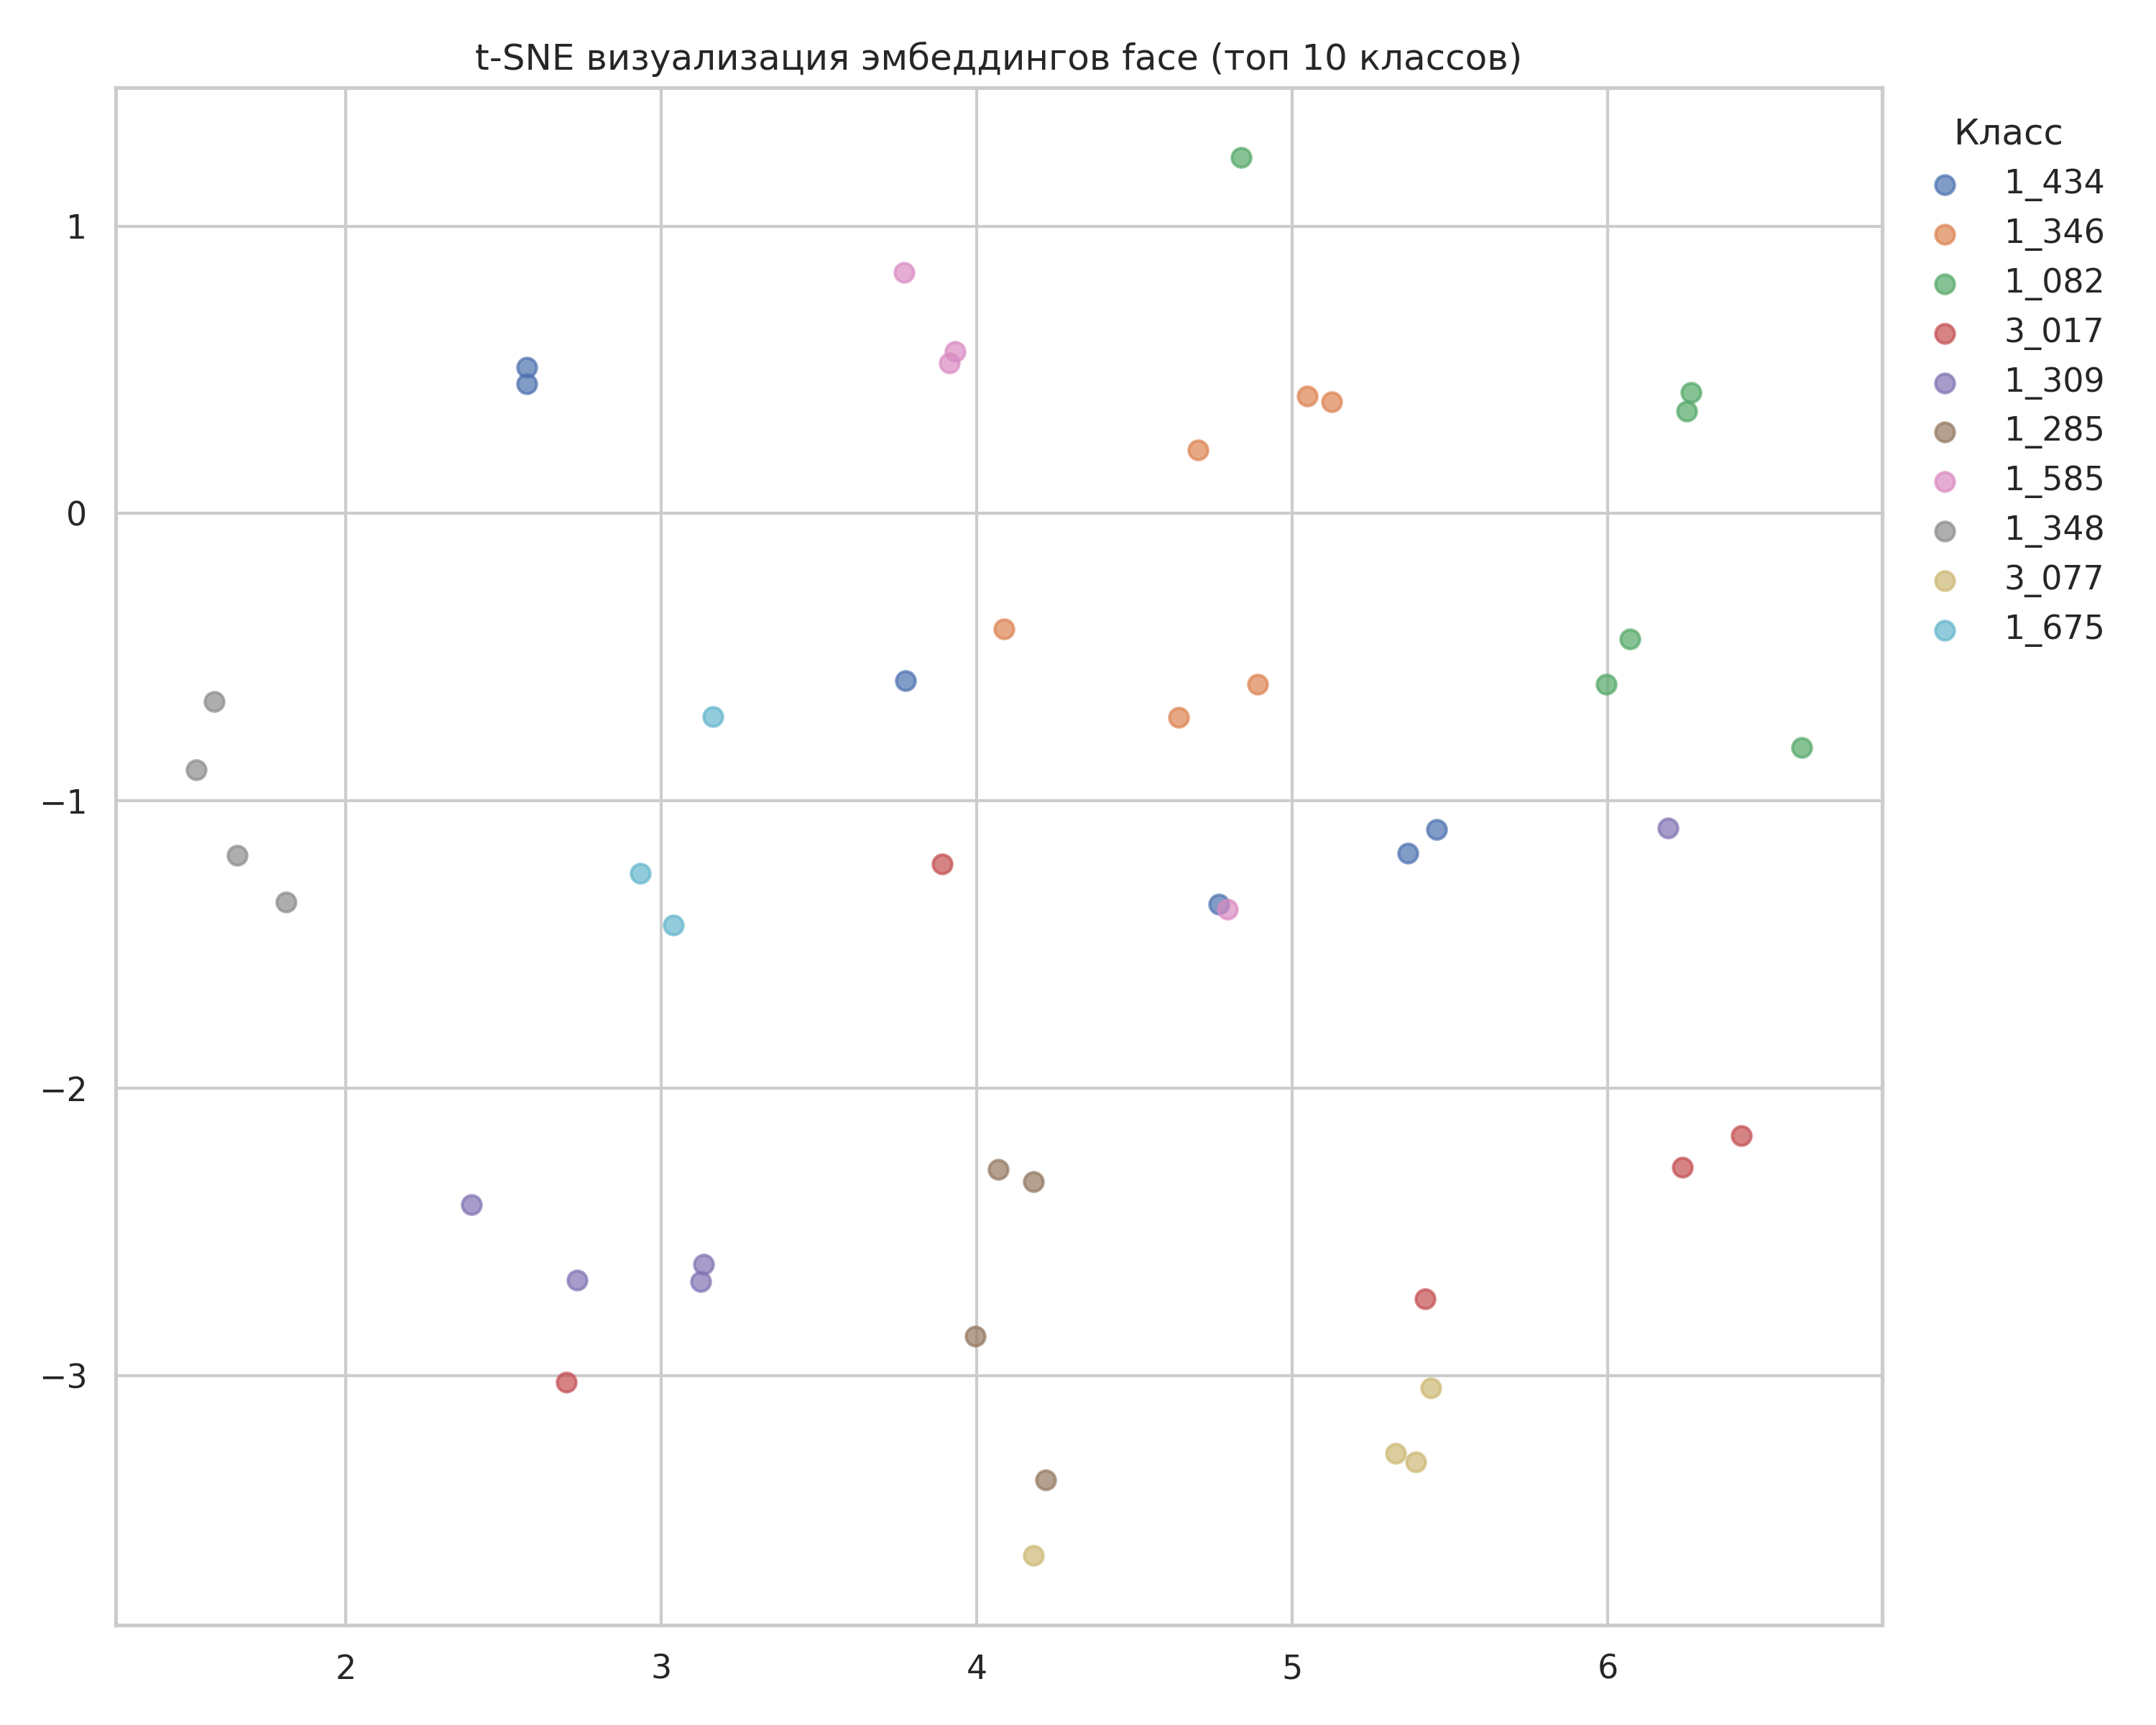
\includegraphics[width=0.8\textwidth]{images/7.png}
\caption{t‑SNE для эмбеддингов лиц}
\label{fig:tsne-face}
\end{figure}

\begin{figure}[H]
\centering
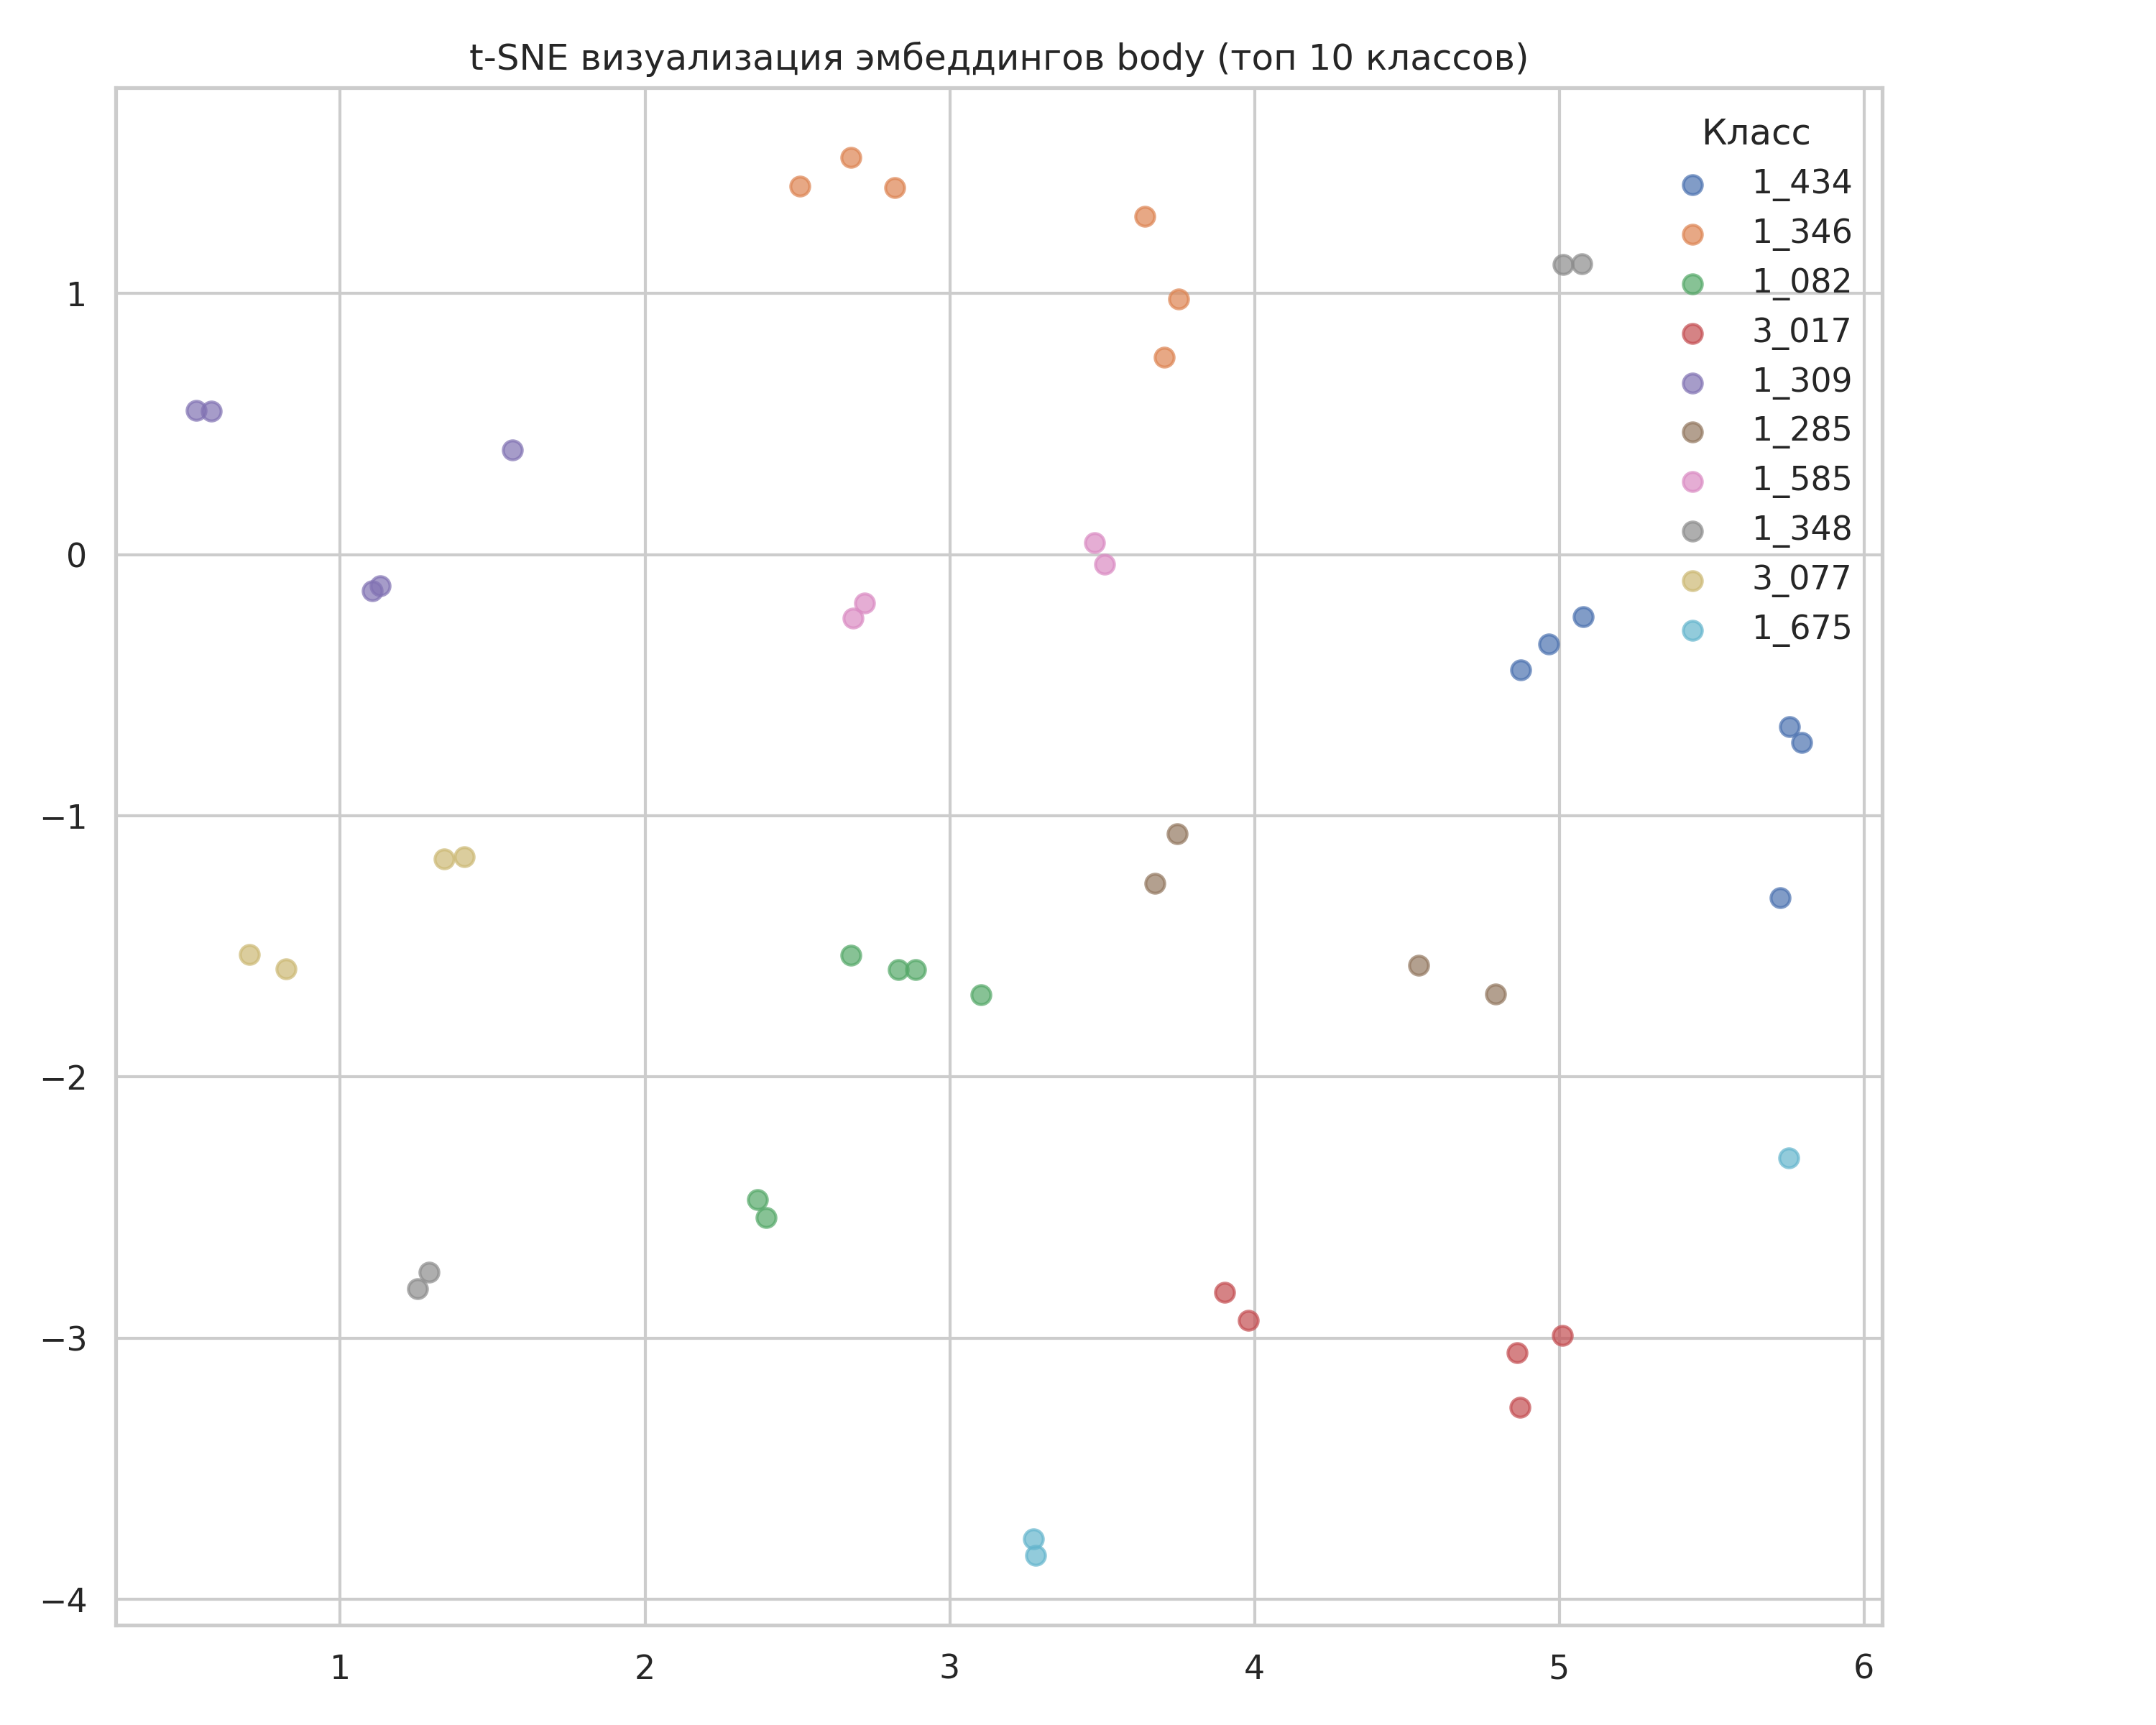
\includegraphics[width=0.8\textwidth]{images/8.png}
\caption{t‑SNE для эмбеддингов силуэтов}
\label{fig:tsne-silhouette}
\end{figure}

\begin{figure}[H]
\centering
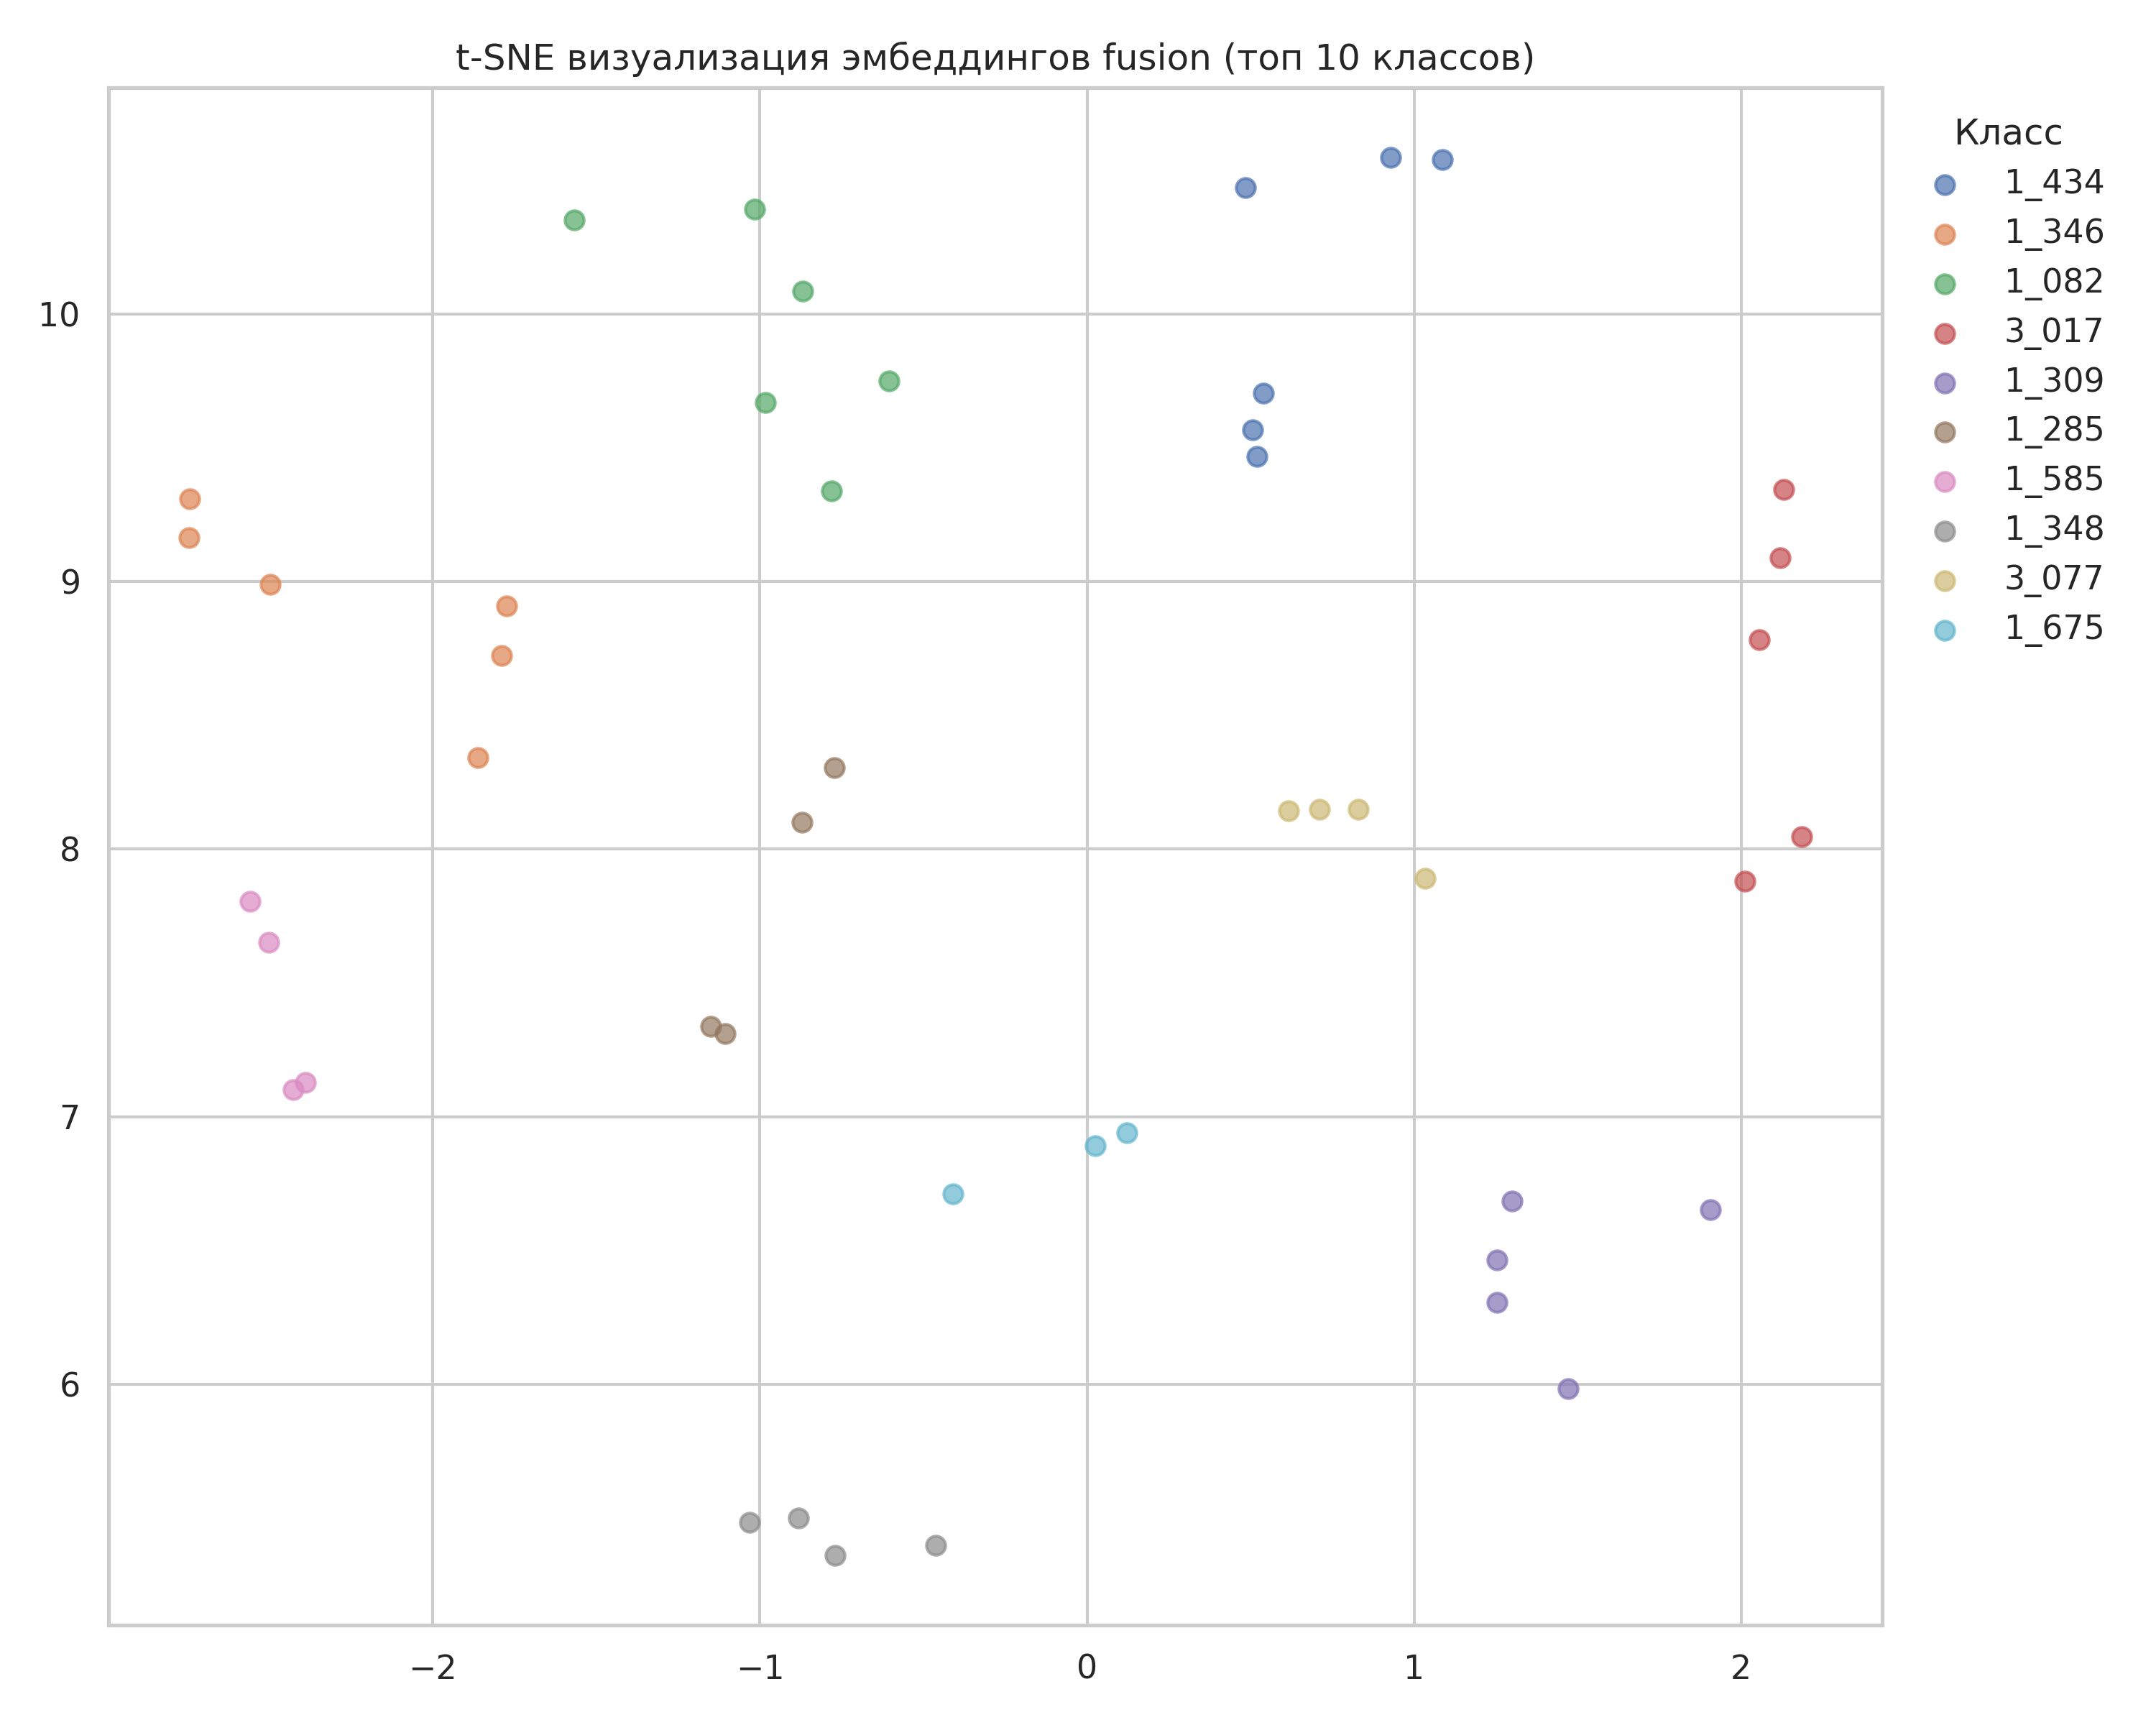
\includegraphics[width=0.8\textwidth]{images/9.png}
\caption{t-SNE для линейного объединения эмбеддингов}
\label{fig:tsne-linear}
\end{figure}

\textit{Эксперименты по~положению~3.} Выполнена оценка итогового качества
многоклассовой реидентификации при использовании предложенной байесовской
интеграции модальностей. Визуализация эмбеддингов методом t-SNE
для байесовского MAP-критерия (рис.~\ref{fig:tsne-bayes}) демонстрирует
устойчивое статистическое разделение классов. Для количественной оценки
построена ROC-кривая (рис.~\ref{fig:roc-curve}) и~рассчитаны стандартные
метрики.

\begin{figure}[H]
\centering
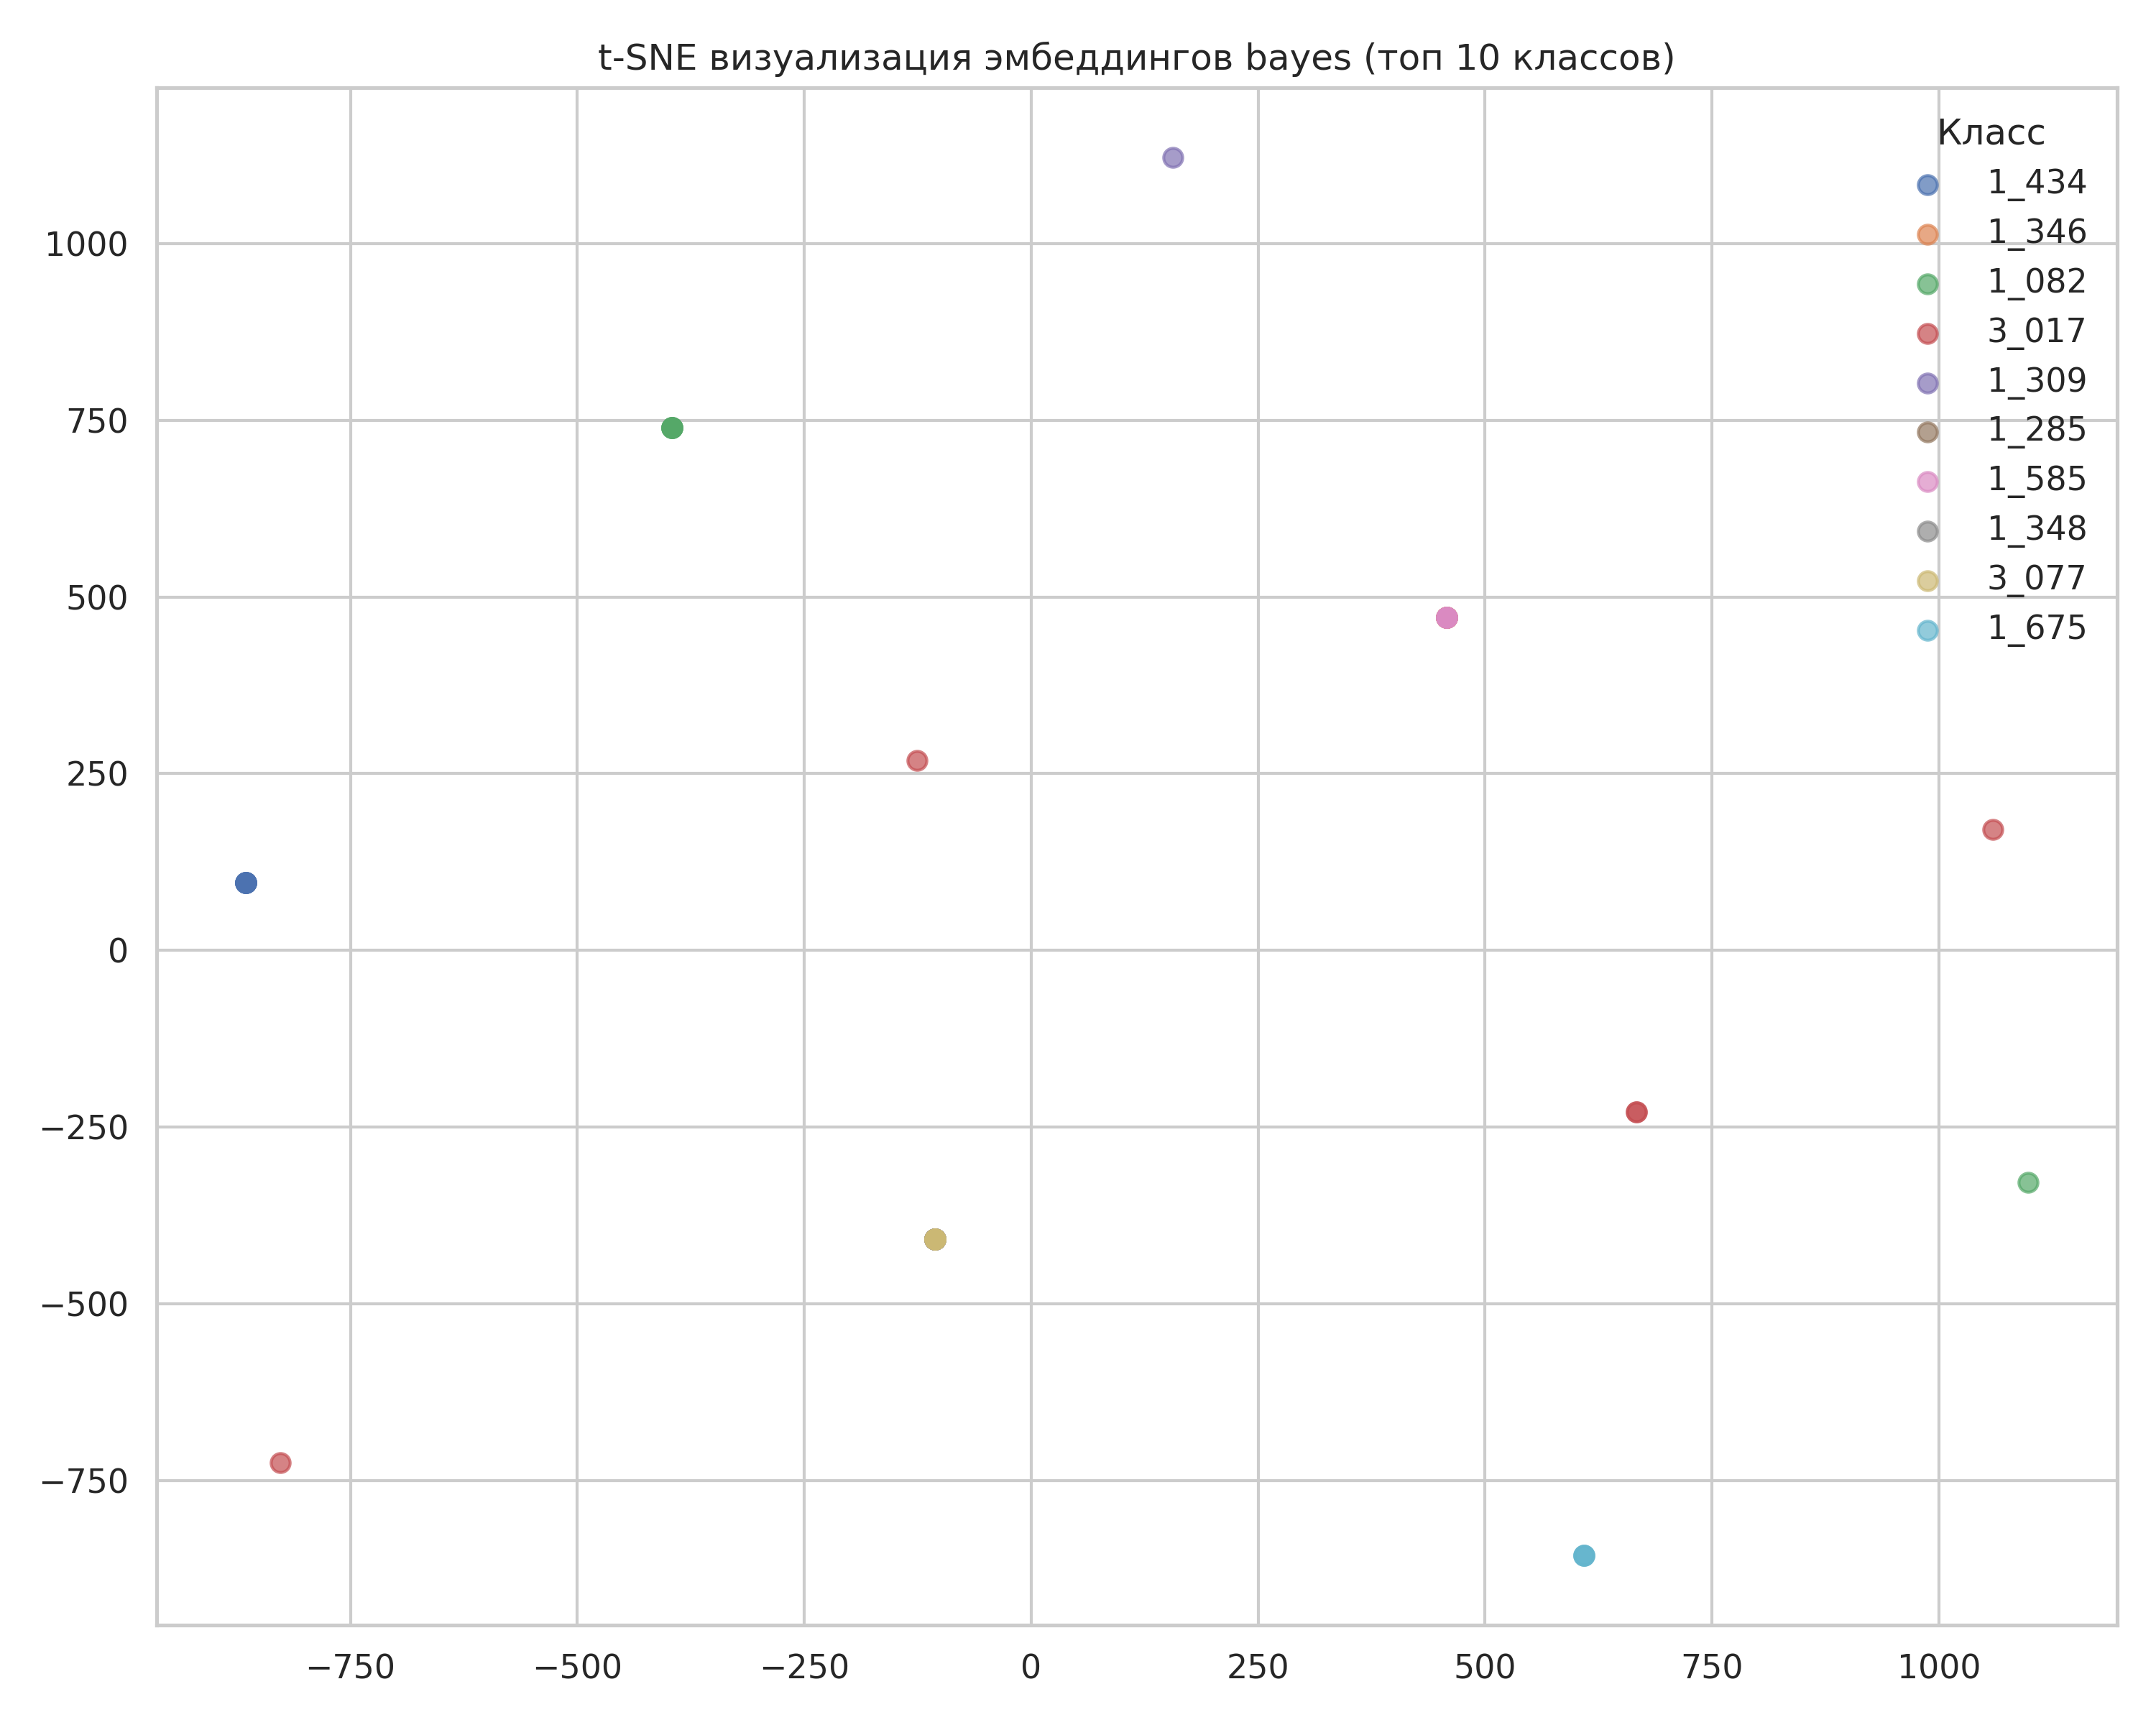
\includegraphics[width=0.8\textwidth]{images/10.png}
\caption{t-SNE для байесовского подхода (MAP-критерий)}
\label{fig:tsne-bayes}
\end{figure}

\begin{figure}[H]
\centering
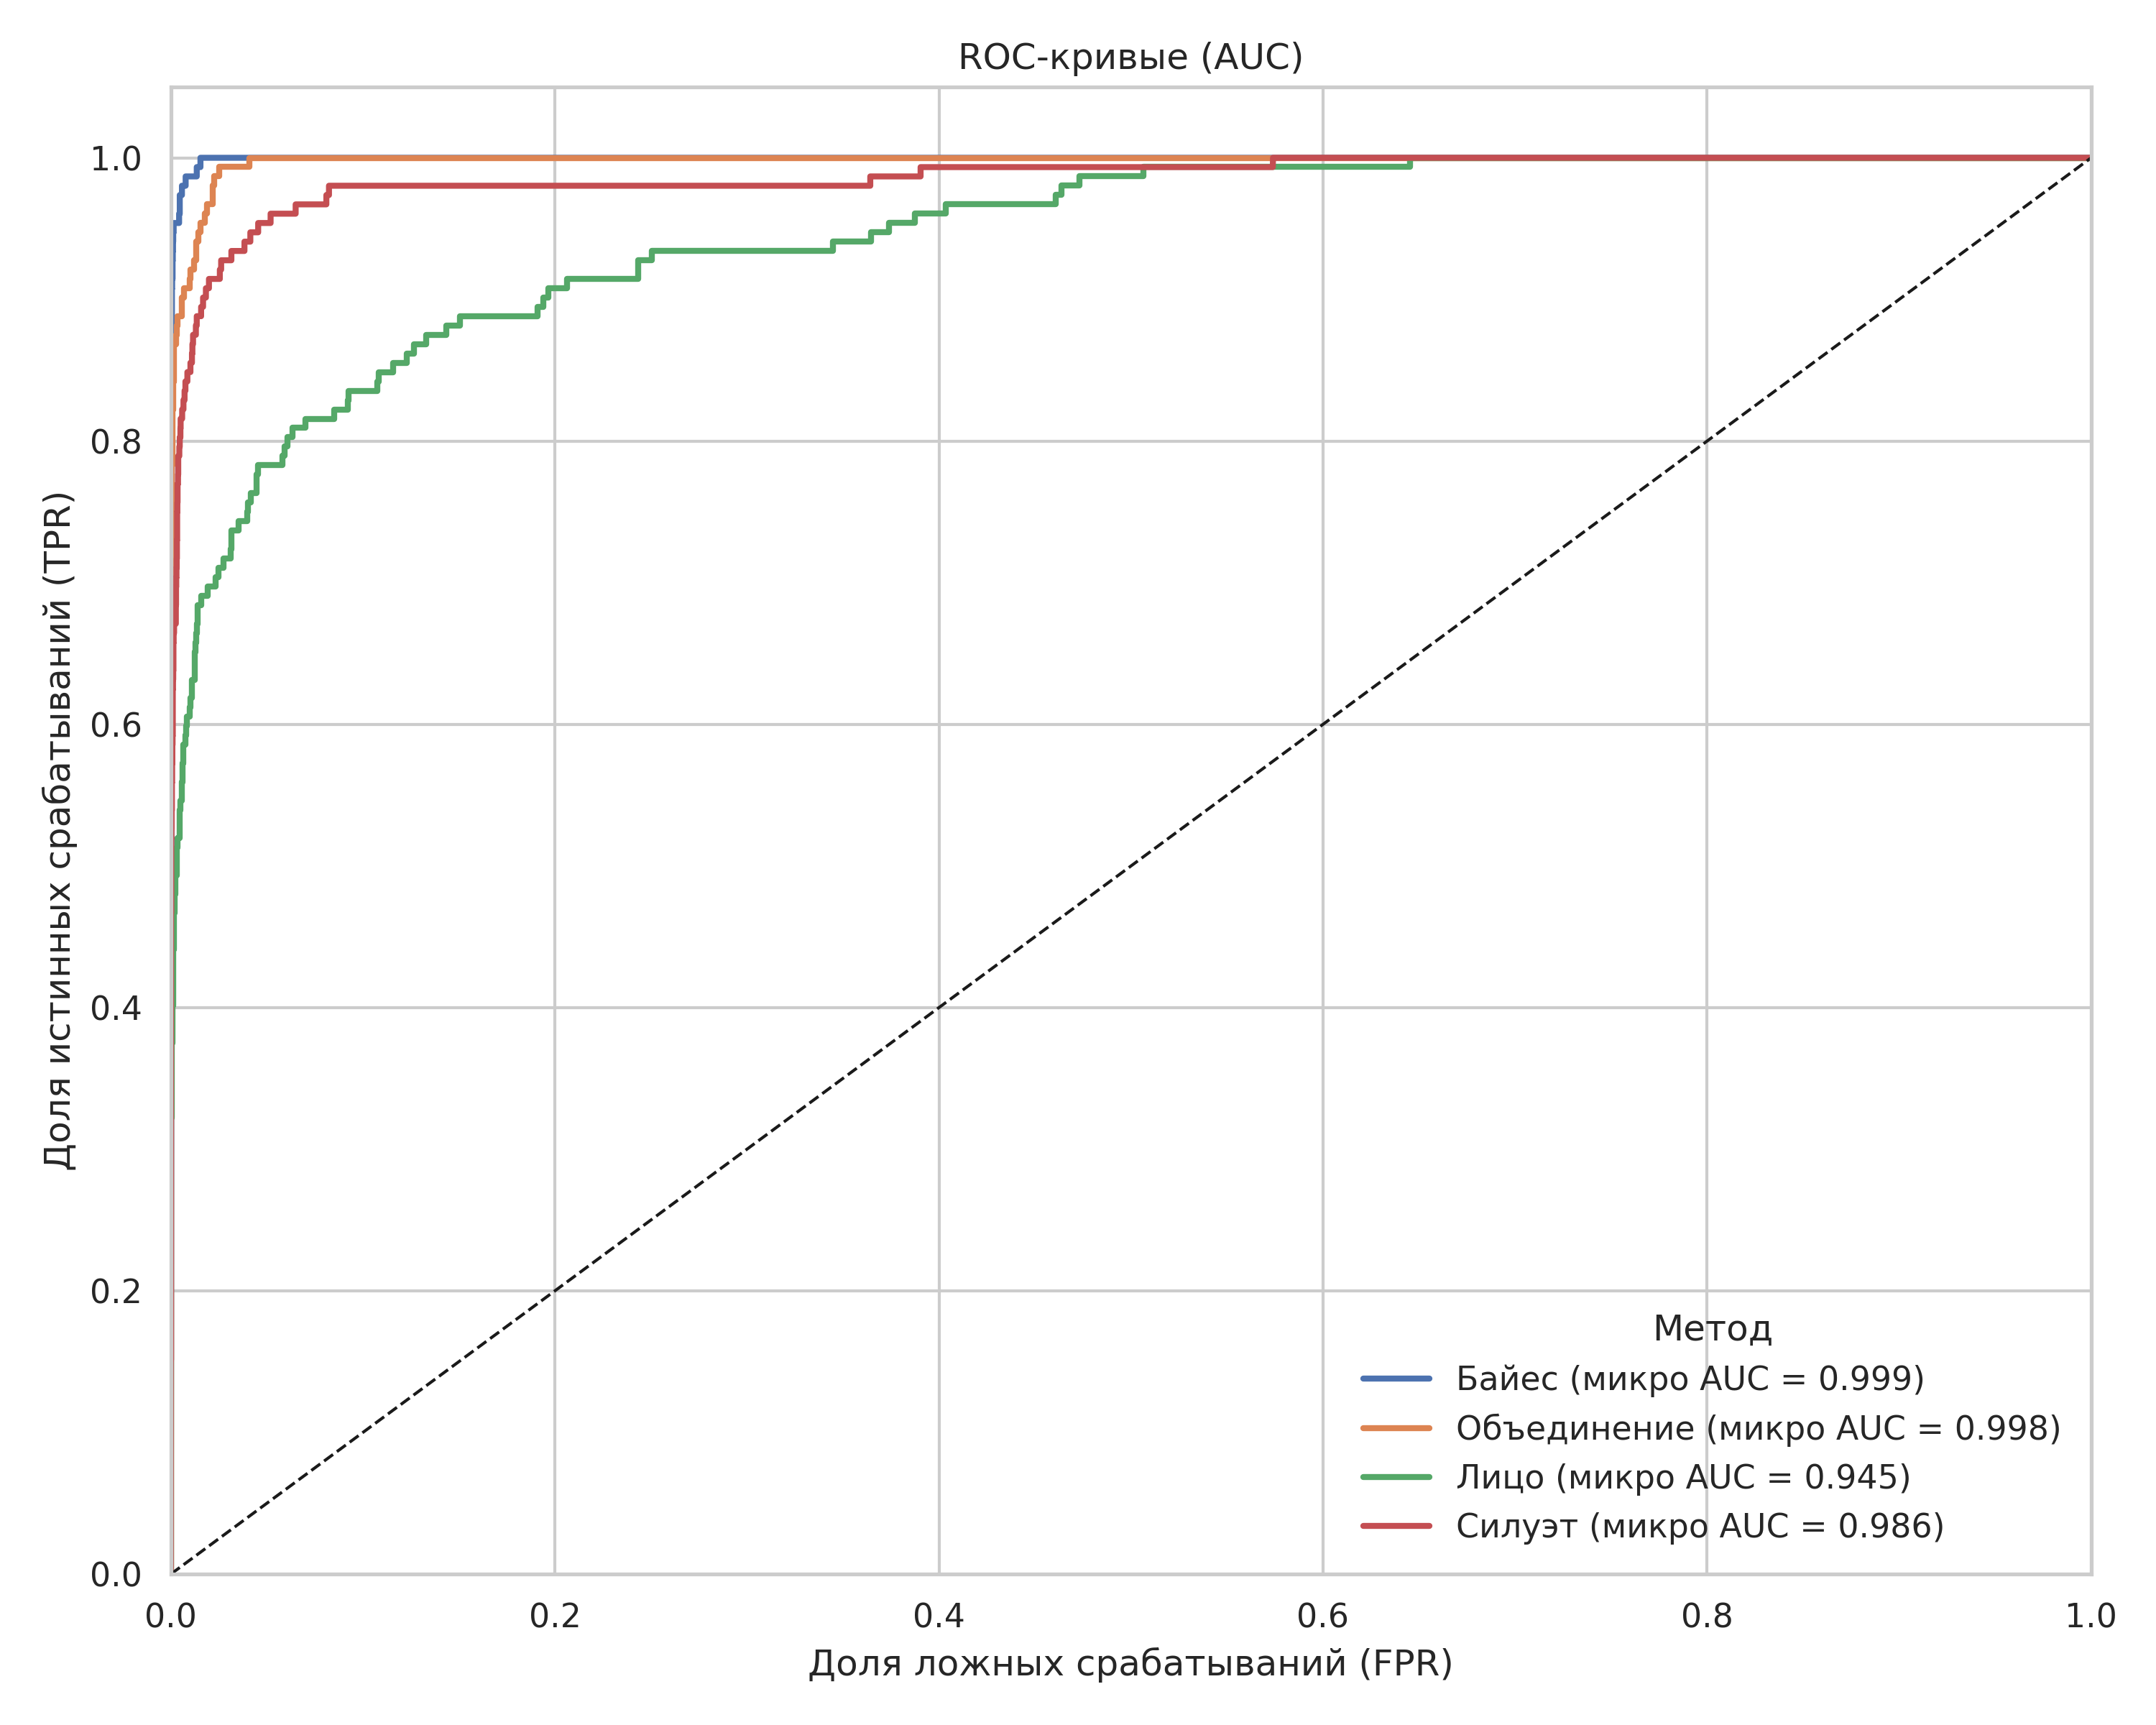
\includegraphics[width=0.8\textwidth]{images/11.png}
\caption{ROC‑кривая}
\label{fig:roc-curve}
\end{figure}

По~результатам вычислительных экспериментов на~наборе CUHK03 получены
следующие macro-усредненные показатели в~постановке многоклассовой
закрытой идентификации (Top-1): Precision~- 95,65\%, Recall~- 95,54\%,
F1-мера~- 94,31\%, Accuracy~- 93,42\%. Для объективного сравнения с~современными решениями
(state-of-the-art) выполнена оценка по~метрике mean average precision~(mAP).
Результаты (табл.~\ref{tab:reid-map}) подтверждают конкурентоспособность
предложенного метода (95,65\%~/~98,3\%~/~89,2\% для
CUHK03~/~Market-1501~/~MARS соответственно).

\begin{table}[H]
\centering
\caption{Сравнение предложенного алгоритма с~state‑of‑the‑art методами
по~mAP,~\%}
\label{tab:reid-map}
\resizebox{\textwidth}{!}{%
\begin{tabular}{lccc}
\hline
Метод & CUHK03 & Market-1501 & MARS \\
\hline
\textbf{Bayesian face\,+\,body (предложенный)} & \textbf{95,65} & \textbf{98,3} & \textbf{89,2} \\
\hline
\multicolumn{4}{l}{\textit{Сравнение на~CUHK03:}} \\
Proposed SGGNN & 94,3 & - & - \\
ProNet++ (ResNet50+RK) & 91,9 & - & - \\
FD-GAN & 91,3 & - & - \\
VI+LSRO & 87,4 & - & - \\
DLCE & 86,4 & - & - \\
UniHCP & 83,1 & - & - \\
Weakly Sup. Pre-train (ResNet50+BDB) & 82,3 & - & - \\
\hline
\multicolumn{4}{l}{\textit{Сравнение на~Market-1501:}} \\
st-ReID & - &98,0 & - \\
SSKD (GH) & - &97,36 & - \\
CLIP-ReID+Pose2ID & - &97,3 & - \\
SOLIDER+UFFM+AMC & - &97,0 & - \\
Unsup. Pre-train (ResNet101+MGN) & - &97,0 & - \\
RGT\&RGPR & - &96,9 & - \\
SOLIDER & - &96,9 & - \\
\hline
\multicolumn{4}{l}{\textit{Сравнение на~MARS:}} \\
B-BOT+OSM+CL Centers (Re-rank) & - &- &88,5 \\
DenseIL & - &- &87,0 \\
PiT & - &- &86,8 \\
FGReID & - &- &86,2 \\
STRF & - &- &86,1 \\
MGH & - &- &85,8 \\
PSTA & - &- &85,8 \\
\hline
\end{tabular}}
\end{table}

\FloatBarrier

%%% Заключение %%%
\pdfbookmark{Заключение}{conclusion}
\section*{Заключение}

В~диссертационной работе решена научно-техническая задача повышения
эффективности информационных процессов автоматического распознавания
и~реидентификации людей в~информационно-поисковых системах, функционирующих
в~режиме, близком к~реальному времени, в~условиях информационной
неопределенности (временная недоступность отдельных модальностей, окклюзии,
шумы и~вариативность наблюдения). Достижение поставленной цели обеспечено
созданием комплексной методики, реализующей единый конвейер обработки:
согласованное детектирование связанных объектов <<силуэт-лицо>>, раздельное
формирование дискриминативных эмбеддингов лица и~силуэта и~их последующую
вероятностную интеграцию при принятии решения.

Основные результаты диссертационной работы заключаются в~следующем:

\begin{enumerate}
    \item Разработана \textbf{комплексная методика} реидентификации людей
    в~информационно-поисковых системах, реализующая единый конвейер
    обработки видеокадра и~включающая четыре последовательных этапа:
    (1)~согласованное детектирование связанных объектов <<силуэт-лицо>>;
    (2)~раздельное извлечение дискриминативных эмбеддингов лица и~силуэта;
    (3)~вычисление гауссовых правдоподобий для каждого класса
    идентификации; (4)~принятие решения по~многоклассовому MAP-критерию.
    Методика интегрирует три разработанных метода (положения~1--3)
    в~единую процедуру и~обеспечивает поэтапное повышение качества
    на~каждой стадии при минимизации каскадного эффекта накопления ошибок.

    \item Разработана модификация критерия обучения детектора (на~базе
    архитектуры YOLOv8) для согласованной локализации топологически связанных
    частей объекта (апробировано на~примере пары \textit{<<силуэт-лицо>>}).
    Метод основан на~введении дополнительного компонента функции потерь
    $\mathcal{L}_{\text{face}}$ и~управляющего коэффициента
    $\lambda_{\text{face}}$, совместно штрафующих ошибки локализации
    лица в~границах силуэта. Экспериментально показано, что подбор
    $\lambda_{\text{face}}$ позволяет повышать метрики обнаружения
    (в~проведенных экспериментах значения в~диапазоне 2,0--2,7 обеспечивают
    наилучшие показатели без существенной деградации по~базовому
    классу).

    \item Предложен метод формирования дискриминативных векторных представлений
    (эмбеддингов) для лицевой и~силуэтной модальностей. Метод включает
    построение специализированных признаковых пространств на~базе ViT-кодировщиков,
    обучение по~функции потерь ArcFace и~$L_2$-нормировку.
    Это обеспечивает получение устойчивых описаний для каждой модальности
    изолированно, минимизируя межклассовые пересечения, что подтверждено
    качественным анализом (визуализация t-SNE).

    \item Разработан метод интеграции лицевых и~силуэтных эмбеддингов
    на~основе байесовской модели и~решающего правила MAP для многоклассовой
    реидентификации. Метод обеспечивает адаптивный вклад каждой модальности
    и~корректное поведение решающего правила при временном отсутствии
    или зашумлении одной из~них без ручной подстройки весов.
    На~наборе CUHK03
    достигнуты macro-усредненные значения: Precision~- 95,65\%,
    Recall~- 95,54\%, F1-мера~- 94,31\%, Accuracy~- 93,42\%; по~метрике
    mAP получены значения 95,65\%/98,3\%/89,2\% на~наборах
    CUHK03/Market-1501/MARS соответственно.

    \item Подтверждена практическая значимость предложенной методики.
    Результаты работы внедрены и~используются в~деятельности ФГБУ~<<НИЦ
    <<Институт имени Н.\,Е.\,Жуковского>>>> (сокращение времени принятия
    решения до~5\% в~системах визуального наблюдения).
\end{enumerate}

Полученные результаты соответствуют паспорту научной специальности~2.3.8
<<Информатика и~информационные процессы>>:
п.~1 (разработка компьютерных методов и~моделей описания, оценки
и~оптимизации информационных процессов)~- в~части компьютерных методов
описания и~оценки процесса реидентификации (математическая постановка,
вероятностная модель интеграции модальностей, решающее правило
на~основе MAP-критерия);
п.~4 (разработка методов и~технологий цифровой обработки аудиовизуальной
информации, извлечения требуемой информации из~изображений
и~видеоконтента)~- в~части алгоритмов обработки видеоконтента:
согласованного детектирования связанных объектов <<силуэт-лицо>>
и~извлечения эмбеддингов лица и~силуэта по~ROI;
п.~13 (разработка и~применение методов распознавания образов, нейросетевых
решающих правил)~- в~части разработанных нейросетевых методов и~правил:
модифицированный детектор YOLOv8 (компонент~$\mathcal{L}_{\text{face}}$
и~коэффициент~$\lambda_{\text{face}}$), двухканальная схема
ViT-кодировщиков (обучаемая по~ArcFace) и~правило по~многоклассовому
MAP-критерию.

Таким образом, предложенная комплексная методика обеспечивает повышение
точности и~устойчивости реидентификации людей в~условиях информационной
неопределенности и~готова к~использованию в~составе высоконагруженных
информационно-поисковых систем при рациональных вычислительных затратах.

%%% Список публикаций %%%
\pdfbookmark{Список публикаций}{publications}
\section*{Список опубликованных работ по теме диссертации}

\subsection*{В~изданиях, входящих в~перечень ВАК при Минобрнауки~РФ:}

\begin{enumerate}
    \item \textbf{Русаков~К.\,Д.} Байесовская модель объединения признаковых
          представлений в~задаче реидентификации личности~// Управление большими
          системами. 2025. Вып.~115. С.~183--202.
    \item \textbf{Русаков~К.\,Д.} Байесовский алгоритм классификации в~задаче
          реидентификации личности~// Известия Юго‑Западного Государственного
          университета. 2025. Том~29, №~3. С.~92--108.
    \item \textbf{Русаков~К.\,Д.}, Генов~А.\,А., Хиль~С.\,Ш. Методика решения
          задачи антиспуфинга по~ограниченному количеству фотографий~//
          Программные продукты и~системы. 2020. Т.~33, №~1. С.~54--60.
    \item \textbf{Русаков~К.\,Д.}, Чехов~А.\,В. Двухэтапный подход
          к~распознаванию коррозии металлических конструкций с~использованием
          сверточных нейронных сетей в~ходе проведения инспекций промышленных
          объектов~// Известия Юго‑Западного Государственного университета. 2021.
          Том~25, №~3. С.~152--166.
\end{enumerate}

\subsection*{В~изданиях, входящих в~базы данных Scopus и~WoS:}

\begin{enumerate}[resume]
    \item \textbf{Rusakov~K.\,D.} Improved Detection of Related Objects on the
          Example of Human Re‑Identification Task~/ Proceedings of the 17th
          International Conference Management of Large‑Scale System Development
          (MLSD). Moscow: IEEE, 2024. P.~\_\_\_\_--\_\_\_\_.
    \item \textbf{Rusakov~K.\,D.} Automatic Modular License Plate Recognition
          System Using Fast Convolutional Neural Networks~/ Proceedings of the
          13th International Conference <<Management of Large‑Scale System
          Development (MLSD)>>. Moscow: IEEE, 2020. P.~1--4.
    \item Rusakov~K.\,D., Seliverstov~D.\,E., Osipov~V.\,V., Reshetnikov~V.\,N.
          Definition of Unique Objects by Convolutional Neural Networks using
          Transfer Learning~// International Journal of Advanced Computer
          Science and Applications. 2020. Vol.~11, Iss.~11. P.~48--54.
    \item \textbf{Rusakov~K.\,D.} Using convolutional neural networks for
          estimating the speed and acceleration of UAVs during takeoff and
          landing through multicamera detection~/ Proceedings of the 16th
          International Conference Management of Large‑Scale System Development
          (MLSD). Moscow: IEEE, 2023. P.~\_\_\_\_--\_\_\_\_.
\end{enumerate}

\subsection*{В~других рецензируемых изданиях:}

\begin{enumerate}[resume]
    \item \textbf{Русаков~К.\,Д.} Использование глубокого обучения
          и~беспилотных летательных аппаратов для мониторинга мусора
          в~прибрежных зонах~/ Труды 14‑го Всероссийского совещания
          по~проблемам управления (ВСПУ‑2024). М.: ИПУ~РАН, 2024. С.~1157--1162.
    \item \textbf{Русаков~К.\,Д.} Подход к~распознаванию утопающих с~помощью
          глубокого обучения~/ Труды 16‑й Всероссийской мультиконференции
          по~проблемам управления (МКПУ‑2023, Волгоград). Волгоград: ВГТУ, 2023.
          №~1. С.~257--259.
    \item Исхакова~А.\,О., \textbf{Русаков~К.\,Д.}, Исхаков~А.\,Ю.,
          Мамченко~М.\,В. Детектирование деструктивного мультимедиа контента
          в~социо‑киберфизической системе мониторинга сети Интернет~/ Труды
          17‑й Всероссийской школы‑конференции молодых ученых <<Управление
          большими системами>> (УБС'2021, Москва). Москва~- Звенигород:
          ИПУ~РАН, 2021. С.~202--212.
    \item \textbf{Русаков~К.\,Д.}, Диане~С.\,А., Россоловский~И.\,А. Алгоритмы
          обработки информации и~управления автономным мультикоптером в~задаче
          мониторинга протяженных объектов~/ Труды 17‑й Всероссийской
          школы‑конференции молодых ученых <<Управление большими системами>>
          (УБС'2021, Москва). Москва~- Звенигород: ИПУ~РАН, 2021.
          С.~490--497.
    \item \textbf{Русаков~К.\,Д.}, Гончаренко~В.\,И., Горелов~А.\,В. Модель
          прогноза технического состояния космического аппарата на~основе
          искусственных модульных нейросетей~/ Труды 19‑й Международной
          конференции <<Цифровая обработка сигналов и~ее применение~-
          DSPA‑2017>> (Москва, 2017). М.: РНТОРЭС имени А.\,С.~Попова, 2017.
          Т.~2. С.~808--813.
\end{enumerate}

\subsection*{Свидетельства о~государственной регистрации ЭВМ:}

\begin{enumerate}[resume]
    \item \textbf{Русаков~К.\,Д.} Программа для реидентификации личности
          на~основе байесовского объединения эмбеддингов лица и~тела:
          Свидетельство о~государственной регистрации программы для ЭВМ
          №~2026617996 РФ; Зарег.~23.03.2026.
    \item \textbf{Русаков~К.\,Д.}, Тевяшов~Г.\,К. Программа для наблюдения,
          захвата рабочей сцены и~детектирования малоразмерных объектов в~их
          тесном скоплении: Свидетельство о~государственной регистрации программы
          для ЭВМ №~2023686143 РФ; Зарег.~04.12.2023.
\end{enumerate}
